\documentclass[letterpaper, 12pt, oneside]{memoir}
\usepackage[no-math]{fontspec}

%%%%%%%%%%%%%%%%%%%%%%%%%%%%%%%%%%%%%%%%%%%%%%%%%%%%%%%%%%%%%%%%%%%%%%%%%%%%%%%
% BEG: PACKAGES
%
\usepackage{amsmath}
\usepackage{caption}
\usepackage{enumitem}
\usepackage{float}
\usepackage[left=1.25in, right=1.25in, top=1.5in, bottom=1.5in]{geometry}
\usepackage{graphicx}
\usepackage{hhline}
\usepackage{hyperref}
\usepackage[all]{hypcap}
\usepackage{newpxtext,newpxmath}
\usepackage{placeins}
\usepackage{siunitx}
\usepackage{subfig}
\usepackage{tcolorbox}
\tcbuselibrary{skins, breakable}
\usepackage{tikz}
\usetikzlibrary{arrows.meta, calc, cd, fadings, positioning, shadings}
\usepackage{url}
\usepackage{xcolor}

\usepackage{Math}
% END: PACKAGES
%%%%%%%%%%%%%%%%%%%%%%%%%%%%%%%%%%%%%%%%%%%%%%%%%%%%%%%%%%%%%%%%%%%%%%%%%%%%%%%

%%%%%%%%%%%%%%%%%%%%%%%%%%%%%%%%%%%%%%%%%%%%%%%%%%%%%%%%%%%%%%%%%%%%%%%%%%%%%%%
% BEG: COLOR/TEXT/FONT CONFIGURATION
%
% \setmainfont{SourceSerifPro-Regular}[
%   BoldFont = SourceSerifPro-Bold,
%   ItalicFont = SourceSerifPro-It,
% ]
% \setsansfont{SourceSansPro-Regular}[
%   BoldFont = SourceSansPro-Bold,
%   ItalicFont = SourceSansPro-It,
% ]
% \setmonofont{SourceCodePro-Regular}[
%   BoldFont = SourceCodePro-Bold,
%   ItalicFont = SourceCodePro-It,
%   Scale = 0.90,
% ]

\definecolor{Orange}{cmyk}{0, 0.40, 0.80, 0}
\definecolor{Red}{cmyk}{0.20, 1.00, 1.00, 0}
\definecolor{LiteRed}{cmyk}{0.01, 0.05, 0.05, 0}
\definecolor{Blue}{cmyk}{1, 0.50, 0.20, 0}
\definecolor{LiteBlue}{cmyk}{0.1, 0.05, 0.02, 0}
\definecolor{Green}{cmyk}{1, 0.50, 0.70, 0}
\definecolor{LiteGreen}{cmyk}{0.1, 0.05, 0.05, 0}
\definecolor{RichBlack}{cmyk}{0.25, 0.25, 0.25, 0.70}

\newtcolorbox[%
  auto counter,%
  number within=chapter%
]{deliverable}[1][]{%
  enhanced,
  colframe=Red,%
  colback=LiteRed,%
  fonttitle=\bfseries,%
  title={Deliverable~\thetcbcounter},
  breakable,
  arc=0pt,
  #1
}
\newtcolorbox[%
  auto counter,%
  number within=chapter%
]{procedure}[1][]{%
  enhanced,
  colframe=Green,%
  colback=LiteGreen,%
  fonttitle=\bfseries,%
  title={Procedure~\thetcbcounter},
  breakable,
  arc=0pt,
  #1
}
\newtcolorbox[%
  auto counter,%
  number within=chapter%
]{definition}[2][]{%
  enhanced,
  colframe=Blue,%
  colback=LiteBlue,%
  fonttitle=\bfseries,%
  title={Definition~\thetcbcounter: #2},
  breakable,
  arc=0pt,
  #1
}

\tikzfading[name=fade lightly right,%
            left color=transparent!0,%
            middle color=transparent!0,%
            right color=transparent!25]

\tikzset{%
  block/.style={%
    rectangle,%
    minimum width=0.5in,%
    minimum height=2.5em,%
    draw=RichBlack,%
    font={},%
    align=center%
  },
  smooth_area_path/.style={%
    dashed,%
    color=RichBlack,%
    line join=round,%
    shorten >=0.025in,%
    rounded corners=0.05in,
    thick,%
  },
  smooth_block/.style={%
    draw=RichBlack,%
    rectangle,%
    rounded corners,%
    thick,%
    minimum width=0.5in,%
    minimum height=2.5em,%
    font={\footnotesize},%
    align=center,%
  },
  smooth_sum/.style={%
    circle,%
    color=RichBlack,%
    minimum width=0.2in,%
    minimum height=0.2in,%
    draw=RichBlack,%
    thick,%
  },
  smooth_path/.style={%
    color=RichBlack,%
    line join=round,%
    shorten >=0.025in,%
    rounded corners=0.05in,
    thick,%
  },
  smooth_annotate/.style={%
    color=RichBlack,%
    font={\small},%
  },
  annotate/.style={%
    font={\small},%
  },
  summer/.style={%
    circle,%
    minimum width=0.2in,%
    minimum height=0.2in,%
    draw=RichBlack,
  },
  signal/.style={%
    color=RichBlack,%
    line join=round,%
    shorten >=0.05em%
  },
  arrow/.style={-{Latex[length=0.5em]}},
  deliverable/.style={%
    draw=RichBlack,%
    rectangle,%
    rounded corners,%
    thick,%
    fill=LiteRed,
    align=center,%
  },
}
%
% END: TEXT/FONT CONFIGURATION
%%%%%%%%%%%%%%%%%%%%%%%%%%%%%%%%%%%%%%%%%%%%%%%%%%%%%%%%%%%%%%%%%%%%%%%%%%%%%%%

%%%%%%%%%%%%%%%%%%%%%%%%%%%%%%%%%%%%%%%%%%%%%%%%%%%%%%%%%%%%%%%%%%%%%%%%%%%%%%%
% BEG: DOCUMENT CONFIGURATION
%

% Chapter Styling
\renewcommand{\chaptername}{Lab}
\chapterstyle{veelo}

%
% END: DOCUMENT CONFIGURATION
%%%%%%%%%%%%%%%%%%%%%%%%%%%%%%%%%%%%%%%%%%%%%%%%%%%%%%%%%%%%%%%%%%%%%%%%%%%%%%%

%%%%%%%%%%%%%%%%%%%%%%%%%%%%%%%%%%%%%%%%%%%%%%%%%%%%%%%%%%%%%%%%%%%%%%%%%%%%%%%
% BEG: DOCUMENT METADATA
%
\hypersetup{
  xetex,
  pdfauthor={Rollen S. D'Souza},
  pdftitle={ECE 380 --- Spring 2020 --- Lab Manual},
  pdfcreator={XeLaTeX with the HyperRef package.},
  breaklinks,
  plainpages=false,
  pdfversion=4,
  pdfduplex={DuplexFlipLongEdge},
  unicode=true,
  pdftoolbar=true,
  pdfmenubar=true,
  pdffitwindow=false,
  pdfstartview={FitH},
  pdfnewwindow=true,
  colorlinks=true,
  linkcolor=Blue,
  citecolor=Green,
  filecolor=magenta,
  urlcolor=Blue,
  linktocpage=true
}

%
% END: DOCUMENT METADATA
%%%%%%%%%%%%%%%%%%%%%%%%%%%%%%%%%%%%%%%%%%%%%%%%%%%%%%%%%%%%%%%%%%%%%%%%%%%%%%%

\begin{document}

%%%%%%%%%%%%%%%%%%%%%%%%%%%%%%%%%%%%%%%%%%%%%%%%%%%%%%%%%%%%%%%%%%%%%%%%%%%%%%%
% BEG: TITLE PAGE
\newgeometry{margin=0.5in, marginparsep=0in}
\thispagestyle{empty}
\begin{titlingpage}
\begin{tikzpicture}[remember picture, overlay, x=1in, y=1in]
  \node[inner sep=0pt, anchor=north west, scope fading=south] at (current page.north west) {%
    \includegraphics[%
      height = 9.5in,%
      trim = 300 20 0 50,
      clip%
    ]{STP-2-Mission-Landing}%
  };

  \node [at={($(current page.north west)+0.5*(1, 0)$)}] (A1) {};
  \node [at={($(current page.south west)+1.0*(1, 0)$)}] (A2) {};
  \node [at={($(current page.south west)+2.0*(0, 1)$)}] (B) {};
  \node [at={($(current page.south east)+0.5*(0, 1)$)}] (C) {};

  \fill [color={Orange}, path fading={fade lightly right}]
    (A1)
    rectangle
    (A2);

  \fill [color={RichBlack}]
    (current page.south west)
    rectangle
    (A1);
  \fill [color={RichBlack}]
    (current page.north west)
    --
    ($(current page.north west) + 1.0*(1, 0)$)
    --
    ($(current page.north west) - 1.0*(0, 1)$)
    --
    (current page.north west);
\end{tikzpicture}
\vfill
\begin{flushright}
{
  \rmfamily\HUGE\noindent
  \textbf{ECE 380 --- Intro to Feedback Control}\\
  Spring 2020\\
  {Lab Manual v0.5}\\
  {
    \scshape
    \small Built \today ---
    \makeatletter
    \small Commit {%
      \@@input|"git rev-list --max-count=1 HEAD | cut -c -6 -"
    }
    \makeatother
  }
}
\end{flushright}
\begin{flushright}
{
  \rmfamily\Large\noindent
  Rollen S. D'Souza
}
\end{flushright}
\vspace{0.25in}
\end{titlingpage}

\restoregeometry

\pagebreak
% END: TITLE PAGE
%%%%%%%%%%%%%%%%%%%%%%%%%%%%%%%%%%%%%%%%%%%%%%%%%%%%%%%%%%%%%%%%%%%%%%%%%%%%%%%

%%%%%%%%%%%%%%%%%%%%%%%%%%%%%%%%%%%%%%%%%%%%%%%%%%%%%%%%%%%%%%%%%%%%%%%%%%%%%%%
% BEG: COPYRIGHT BS
%
\thispagestyle{empty}
%\noindent\textcopyright 2020 Rollen S. D'Souza\\

\noindent
Cover page image captured by SpaceX\textregistered~on their
STP-2 Mission, licensed under the Creative Commons Non-Commercial 2.0. See
\href{https://www.flickr.com/photos/spacex/48129269942/}{here}
for original content. It is, of course, a photo of one of their self-landing
booster rockets attempting a landing. If you are interested, see the discussion
by Lars Blackmore on \emph{Autonomous Precision Landing of Space Rockets}
in
\href{http://www.larsblackmore.com/nae_bridge_2016.pdf}{this publication}. It
isn't very technical but you can find where to jump from there if you want a
little more technical content.
\begin{center}
  * \qquad * \qquad *
\end{center}
\noindent
A big thank you to
\begin{itemize}[label={}]
  \item{Carmen Caradima,}
  \item{Prof. Christopher Nielsen,}
  \item{Prof. Andrew Heunis,}
\end{itemize}
and other ECE 380 lab and course instructors whose work has inspired much
of this lab manual. This lab manual is just a variation of past
ECE 380 labs. Thank you to Prof. Derek Rayside whose general teaching
style inspires the variations made in this lab.
\begin{center}
  * \qquad * \qquad *
\end{center}

\pagebreak
% END: COPYRIGHT BS
%%%%%%%%%%%%%%%%%%%%%%%%%%%%%%%%%%%%%%%%%%%%%%%%%%%%%%%%%%%%%%%%%%%%%%%%%%%%%%%

\frontmatter

\tableofcontents*
\thispagestyle{empty}

\clearpage
\listoffigures*

\clearpage
\listoftables*

%%%%%%%%%%%%%%%%%%%%%%%%%%%%%%%%%%%%%%%%%%%%%%%%%%%%%%%%%%%%%%%%%%%%%%%%%%%%%%%
% BEG: INTRODUCTION
%
\chapter{Introduction}
Welcome to your remote lab for ECE/SE 380, Introduction to Feedback Control.
The lab portion of this course was designed to give you a hands-on
feel for control using analog circuits. Given the current climate, this is
clearly not possible in the way previously envisioned.

We persist. This lab is designed to run in MATLAB and Simulink. You will engage
in understanding, developing, executing and analyzing Simulink
diagrams that model and simulate control systems. Every lab is
provided with brief motivation on how one can see this applied in a real
world problem. I hope I can help connect the abstract block diagrams of
Simulink with the real world for you.

Control systems is a very broad topic with a long history that even predates
the ideas discussed in this course. This course and lab covers the very basic
notion of control, the idea of the negative feedback loop, buttressed by
the mathematical tools of linear dynamical systems.

\section{MATLAB and Simulink}
MATLAB is a desktop numerical and symbolic
mathematics computing environment. We will not rely heavily on MATLAB
scripting itself and instead use Simulink but you should be familiar with
both environments. Please ensure that, when you are installing MATLAB, you
install
%
\begin{enumerate}[label=(\arabic*)]
  \item{
    MATLAB,
  }
  \item{
    Simulink,
  }
  \item{
    the Control Systems Toolbox,
  }
  \item{
    the Simulink Control Design,
  }
  \item{
    the DSP System Toolbox,
  }
  \item{
    the Signal Processing Toolbox,
  }
  \item{
    the Statistics and Machine Learning Toolbox and
  }
  \item{
    the Symbolic Math Toolbox.
  }
\end{enumerate}
%
Simulink is an add-on to MATLAB that allows you to design and simulate
systems (physical or otherwise) using block diagrams like in
Figure~\ref{fig:intro:1}.
%
\begin{figure}[H]
  \centering
  \begin{tikzpicture}[x=1in, y=1in]
    \node [draw, block] (Controller) {\(K_p + K_i\frac{1}{s}\)};
    \node [draw, block, right=0.5 of Controller] (Plant) {\(\frac{1}{s}\)};
    \node [draw, summer, left=0.5 of Controller] (Sum) {};
    \node [below=0.5 of Sum] (BelowSum) {};

    \draw [arrow, signal]
      (Controller.east) -- (Plant.west);
    \draw [arrow, signal]
      (Plant.east)
      --
      +(0.35, 0)
      |-
      (BelowSum.base)
      --
      (Sum.south)
      node [below right, annotate] {\(-\)};
    \draw [arrow, signal]
      (Sum.east) -- (Controller.west);
    \draw [arrow, signal]
      ($(Sum.west)+1*(-0.5, 0)$) -- (Sum.west);
    \draw [arrow, signal]
      (Plant.east) -- +(0.7, 0);
  \end{tikzpicture}
  \caption[Example Feedback Diagram]{
    Example feedback diagram. The blocks are differential equations, expressed
    as a Laplace transfer function, that take an input signal and produce an
    output signal.
  }
  \label{fig:intro:1}
\end{figure}
%
Figure~\ref{fig:intro:1} can be replicated perfectly in Simulink.
That fact makes it easy for engineers to quickly design and verify
control designs. Simulink even supports direct interaction with
hardware but we will not utilize this feature.

The core of Simulink is the notion of a \emph{block}, maps that take an input
signal and produce an output signal.
The blocks we'll be concerned with primarily are \emph{gains}
(multiplier) depicted in Simulink like
\begin{center}
  \begin{tikzpicture}[x=1em, y=1em]

    \draw
      (0, 0)
      --
      (3, 1)
      --
      (0, 2)
      --
      (0, 0)
      --
      (3, 1)
      node [at={(1, 1)}] {\(K\)};

  \end{tikzpicture}
\end{center}
and \emph{transfer functions} depicted in Simulink like
\begin{center}
  \begin{tikzpicture}[x=1em, y=1em]

    \node [draw, block] (Plant) {\(\frac{s+1}{s+2}\)};

  \end{tikzpicture}.
\end{center}
You may be provided template blocks to help you setup the Lab plant, the
system we wish to control; it will then be your task to analyze this block,
design a controller, and implement it by linking up blocks
in the appropriate feedback architecture.

\section{Lab Logistics and Deliverables}\label{intro:logistics}
Lab deadlines can be found in your course outline and on LEARN.
Read carefully.
Times are provided in the active Eastern Time.
Every lab requires you to complete a number of procedures described in green boxes like
\begin{procedure}[]
  Here are some steps:
  \begin{enumerate}[label=(\arabic*)]
    \item{Yes here is step 1,}
    \item{oh wow step 2,}
    \item{you got the idea.}
  \end{enumerate}
\end{procedure}
\noindent
and deliverables described in red boxes like
\begin{deliverable}[]
  Here are some things you will need to save for your report.
\end{deliverable}
Procedures are simply steps you should follow that will eventually result in one or more deliverables, namely something you must record and submit as part of your report. {\color{red}Note that the sequential number of the procedure may differ from the number of the deliverable. Procedures are, nevertheless, positioned and numbered such that they integrate well in the flow of information of specific sections. In other words, do not skip content trying to jump from a deliverable to what you may think is the corresponding procedure simply based on the procedure's number.}\\

Every lab chapter ends with a final summative deliverable, usually
consisting of a series of questions that you must answer.
%
All the deliverables should be packaged up in an organized way; ideally
they should be in your report in the order presented under headings directly corresponding to the deliverable label (1.1, 1.2, etc.). \\

We expect that the majority of your submissions will be typeset. However, for parts that involve a lot of formulas/diagrams/equations, it is acceptable to include \textbf {neatly hand-written parts}; make sure that they are \textbf {organized and legible}.
Your final report must be submitted as one PDF document on Learn; it is the duty of both lab partners to verify that the PDF file has been rendered correctly.
Your grade is entirely based on your report.\\

Occasionally, there has been confusion about what is allowed and what is not allowed in labs. You are responsible for knowing what constitutes an "academic offence" according to \href{https://uwaterloo.ca/secretariat/policies-procedures-guidelines/policy-71} {Policy 71} of the university. In particular, according to this policy:
\begin{enumerate}
\item{Cheating is an academic offence. Cheating includes copying from another student's work or allowing another student to copy from one's own work, submitting another person's work as one's own, fabrication of data and use of unauthorized aids.}
\item{Plagiarism (the act of presenting the ideas, words, or other intellectual property of another as one's own) is an academic offence. The use of other people's work must be completely and unambiguously acknowledged and referenced in all written material, including laboratory reports and computer programs.}
\end{enumerate}

In this course, labs are being done in groups of two students, subject to enrolment constraints. Each group must do their own analysis and their own design, do their own edits to the Matlab/Simulink files provided, and write up their own lab report. However:
\begin{enumerate}
\item{You may talk to the lab instructor, the teaching assistant and the course instructor about any aspect of the lab.}
\item{You are allowed to consult with other students in the class or share \emph{high-level ideas and approaches}, but \emph{not} to share detailed analysis or detailed design results.}
\item{You may not obtain or look at lab reports (either in hardcopy or softcopy) written by other students, whether they are current students or former students of ECE/SE 380. You may not let any other student access any part of your lab report (either in hardcopy or softcopy).}
\item{In your report, you must completely and unambiguously acknowledge and reference any person, website, report, book, or notes that you used to help you with your work. You should reference this lab manual, and the course notes, for example.}
\item{You must include in each report, and sign, the following statement:}
\end{enumerate}

\begin {declaration} \label{intro:decl} \hypertarget{intro:decl}
  We acknowledge and promise that: 
  \begin{enumerate}[label=\emph{\alph*})]
  \item We are the sole authors of this lab report and associated simulation files/code.
  \item This work represents our original work.
  \item We have not shared detailed analysis or detailed design results, computer code, or Simulink diagrams with any other student.
  \item We have not obtained or looked at lab reports from any other current or former student of ECE/SE 380, and we have not let any other student access any part of our lab work.
  \item We have completely and unambiguously acknowledged and referenced all persons and aids used to help us with our work.
  \end{enumerate}
  Student1 Name and Signature:\\
  Student2 Name and Signature: 
\end{declaration}

Every lab has its own grading scheme, but the following penalties apply equally to all labs:
\begin{itemize}
  \item{
    \(-5\%\) for poor organization or hand-written parts that are messy or difficult to read,
  }
  \item{
    \(-5\%\) for the submission not being in PDF format,
  }
  \item{
  	\(-5\%\) for not including the \hyperlink{intro:decl}{Declaration of Authorship} shown above,}
  \item{
    \(-1\%\) per hour within the first 24 hours past the submission deadline. After 24 hours, the penalty becomes \(-100\%\). If prior arrangements are made or a valid reason presented within one week from the missed deadline, the late penalty is waived. In no case will a lab report be accepted more than one week past the deadline. If a valid reason exists for being unable to hand in the lab report
    within the week following the deadline, then a solution tailored to each particular situation will be offered.  \textbf{Contact the Lab Instructor for this.}
    All reports are due at \texttt{23:59 Eastern Time} on the due date shown in the Course Outline.
   }
\end{itemize}
Minor mistakes are penalized quite steeply so check your work.
Mistakes in discussions usually amount to theoretical mistakes in understanding;
we will make an attempt to avoid double, or any other cascade, deduction.

% END: INTRODUCTION
%%%%%%%%%%%%%%%%%%%%%%%%%%%%%%%%%%%%%%%%%%%%%%%%%%%%%%%%%%%%%%%%%%%%%%%%%%%%%%%

\mainmatter
\chapter{System Identification Fundamentals}\label{Lab:1}
Low-pass filters are ubiquitous. They can be found in the hardware of
audio processing chips, or the software of image editing tools. As you may
recall from a course on Signals and Systems theory\footnote{If you haven't
taken a course in Signals and Systems, speak to your Lab Instructor on
knowledge you may be lacking.}, a low-pass filter
is a system that, generally speaking, rejects high-frequency signals while
``passing through'' low-frequency signals. In this lab you will be asked
to analyze a low-pass filter block and determine its parameters via a time
domain approach. This is not meant to be a difficult lab and is instead
designed to give you a sense of the lab format. However, it will put to the
test your knowledge of signals and systems. If you have forgotten your
Laplace transforms, this is a good time to remind yourself of them!

In the real world, our models are rarely perfect. The techniques
you learn here generalize nonetheless. Whenever you confront a novel system,
devise a generic model that you think characterizes its behaviour and then
come up with experiments that expose its characteristics; this gives you
estimates of the generic model's parameters that best fit the actual system.
We will encounter such a situation in a future lab.

\section{Objectives}
The primary objectives of this lab are to
\begin{enumerate}[label=(\arabic*)]
  \item{
    \textbf{Install} MATLAB, Simulink and required toolboxes.
    Alternatively, \textbf{connect remotely} to
    \url{engterm.uwaterloo.ca} or any other lab computer of your choice
    that has MATLAB.
  }
  \item{
    Understand how to \textbf{open} and \textbf{modify}
    a Simulink diagram and how to run a simulation.
  }
  \item{
    Understand how to \textbf{log} signals for future inspection.
  }
  \item{
    Understand how to \textbf{plot} figures and capture them.
  }
  \item{
    Understand the theory behind first-order low-pass systems.
  }
  \item{
    Understand how to \textbf{identify} a first-order low-pass system.
  }
\end{enumerate}
This is not a particularly long lab, but you may have trouble as it is
very likely your first encounter with Simulink. As a result, I suggest you
give you and your partner time to work through the lab and the problems.
I also recommend you spend some time by yourself exploring Simulink so as to
reduce the amount of time you spend on future labs.

\section{Experimental Procedure}
This entire lab will be done using the ``\texttt{Lab\_1.slx}'' Simulink model.
First extract the ``\texttt{Lab\_1\_Data.zip}'' file available from Learn.
Inside there you will find zip files created for each individual group. Extract
the zip file associated to your group, and there you will find the relevant
``\texttt{Lab\_1.slx}'' file. The R2018 version may be found in a nested
directory.

In the Simulink model you will
find a number of blocks already placed for you in an open loop configuration:
\begin{itemize}
  \item{a signal generator,}
  \item{a summing junction,}
  \item{an adjustable gain block,}
  \item{a ``plant'', the system we are going to analyze, and}
  \item{a terminator.}
\end{itemize}
%
The plant --- labelled \(P(s)\) in the diagram --- can be assumed to be a
transfer function taking the form
\[
  P(s) = \frac{b T}{s + a T} \quad ,
\]
where \(a, b > 0\) and \(T \in \{10, 100\}.\) Your goal is to use the
techniques described in the following subsections to estimate the parameters
\(a,\) \(b\) and \(T\) for your plant. This process is known as
\textbf{system identification} and it is a critical precursor to control
design. How can we design a controller if we don't even know the parameters
of the system we wish to control?

\subsection{Acquiring the Bandwidth in Time-Domain}
The goal of this portion of the lab is to acquire the bandwidth of the
given linear system. What is the bandwidth? To understand and acquire it,
we must first know what the DC gain of a system is.
%
\begin{definition}[label={def:lab1:dcgain}]{DC Gain}
  Let \(G(s)\) be a \emph{stable} transfer function
  that maps an input signal \(U(s)\) to an
  output \(Y(s).\) The \textbf{DC gain} of \(G(s)\) is \(G(0)\) and,
  if \(u(t) = A \mathbf{1}(t)\) for \(A \in \Real,\) it satisfies the relation
  \[
    \lim_{t\to \infty} y(t) = A G(0).
  \]
\end{definition}
%
Observe that the DC gain \(G(0)\) is called precisely that because when we
apply a square (DC-like; step) signal change, the system's output converges
to the amplitude of the input times \(G(0).\)
%
Instead of computing the DC gain by evaluating the system's response to a step
input, we take a different approach.
%
\begin{procedure}[label={proc:lab1:p1}]
  You will acquire the DC gain of the plant \(P(s)\). Follow these steps:
  \begin{enumerate}[label=(\arabic*)]
    \item{
      \textbf{Open} the signal generator block, \textbf{set} the type of signal
      to be a sinusoidal wave, and set the
      \textbf{amplitude} to be \(1\) and the \textbf{frequency}
      to be \(\SI{0.5}{Hz}.\) This signal is so low frequency that it
      emulates a constant signal.
    }
    \item{
      \textbf{Run} the script \texttt{generate\_lab\_1\_plot.m} and inspect
      Figure 1, which depicts the input and output signal.
    }
    \item{
      \textbf{Measure the peak to peak amplitudes} of the input and output signals respectively when the system is in steady-state.
    }
    \item{
      \textbf{Estimate} the DC gain by dividing the output amplitude
      by the input amplitude. \emph{Remember, we chose the input amplitude
      to be \(1\)!}
    }
  \end{enumerate}
\end{procedure}
%
\begin{figure}
  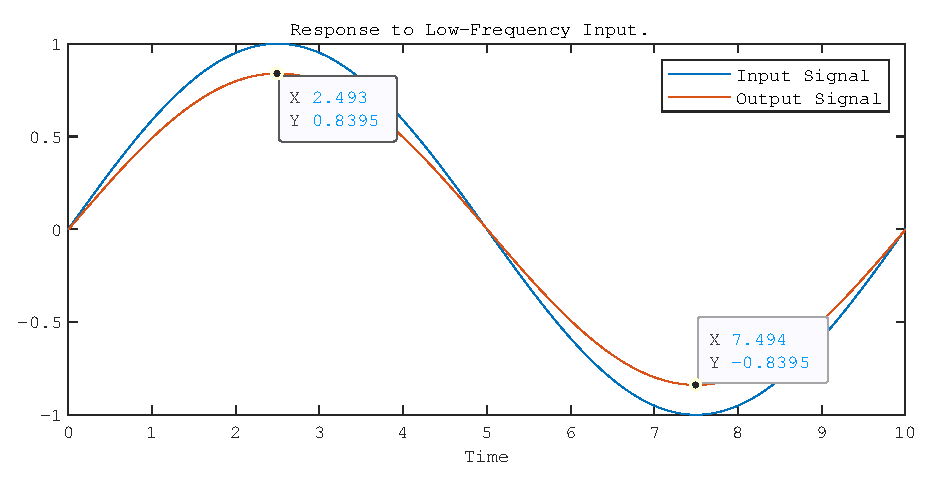
\includegraphics{images/Lab_1_LowFrequency.eps}
  \caption[Low Frequency Response of a Low-Pass Plant]{The low-frequency response to my low-pass plant \(P(s).\) The gain
  at this low frequency is \(0.8395.\) Can you see why? What is the DC
  gain approximately?}
  \label{fig:lab1:lowfreq}
\end{figure}
%
\begin{figure}
  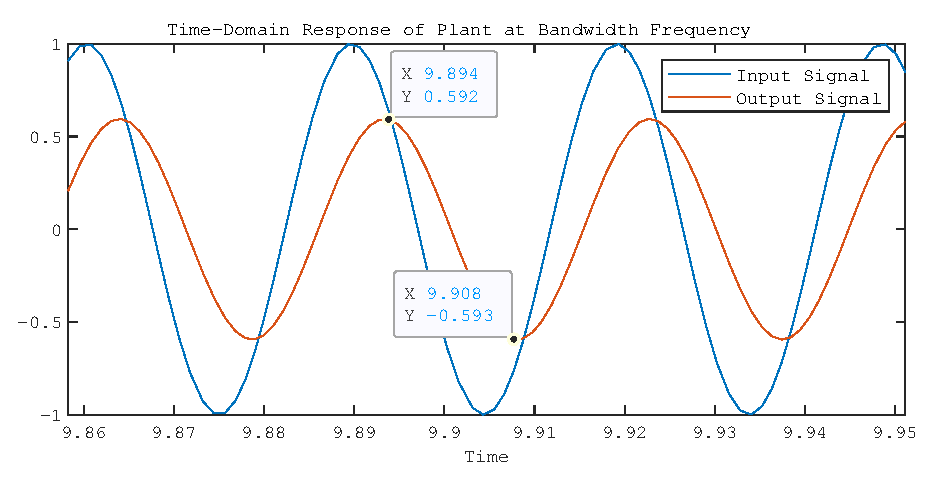
\includegraphics{images/Lab_1_Bandwidth.eps}
  \caption[Time-Domain Response of a First-Order System at the Bandwidth Frequency]{The response to my \(P(s)\) at the bandwidth frequency.
  Can you see why this is the bandwidth frequency for my plant?}
  \label{fig:lab1:bandwidth}
\end{figure}
%
\begin{deliverable}[label={lab1:d1}]
  \textbf{Record} your estimated DC gain and \textbf{capture} the generated
  figure with the cursors you used to measure the amplitudes.
  Your figure should like Figure~\ref{fig:lab1:lowfreq}.
\end{deliverable}
%
For low-pass systems, as we increase the frequency of the input, we will
observe, the output amplitude \emph{decreases}. The bandwidth frequency
is the frequency that marks the point where we distinguish between the
``low'' frequency inputs a low-pass system sustains and the ``high'' frequency
inputs a low-pass system rejects.
%
\begin{definition}[]{Bandwidth}
  Let \(G(s)\) be a proper transfer function
  that maps an input signal \(U(s)\) to an output \(Y(s).\)
%
  Say the input is a sinusoid of the form \(A \cos(\omega t)\) with amplitude
  \(A.\) In steady-state, the amplitude of \(y(t)\) converges to a constant
  \(B.\) The \textbf{gain at frequency \(\omega\)} is
  \(\left\|G(j\omega)\right\| = \frac{B}{A}.\)
%
  The \textbf{bandwidth (frequency)} of \(G(s)\) is the \emph{smallest}
  frequency \(\omega\) which satisfies
  \[
    \frac{1}{\sqrt{2}} = \frac{\left\|G(j\omega)\right\|}{\left\|G(0)\right\|}.
  \]
\end{definition}
%
What is the definition above trying to characterize? The
gain is the multiplier between the input amplitude and output amplitude. For
a low-pass system, this gain decreases as a function of input frequency. The
bandwidth frequency is the frequency where this gain has fallen, in comparison
to the DC gain, by factor of \(\sqrt{2}.\) This is further demonstrated
by the difference in response we observe between Figure~\ref{fig:lab1:lowfreq}
and Figure~\ref{fig:lab1:bandwidth}. Note how much smaller the output signal
is in the response with higher frequencies in comparison to the response
with lower frequencies.
%
\begin{procedure}[label={proc:lab1:p2}]
  You will acquire the bandwidth frequency of the plant \(P(s)\).
  Follow these steps:
  \begin{enumerate}[label=(\arabic*)]
    \item{
      \textbf{Predict} the amplitude of the steady-state output at the
      bandwidth frequency. As an example, if your DC gain is \(0.8395\) then
      the ratio between the input signal amplitude and the output signal
      at the bandwidth frequency is
      \[
        \frac{0.8395}{\sqrt{2}}.
      \]
      If my input signal has amplitude \(1,\) then I should look for
      an output signal amplitude with the above value.
    }
    \item{
      \label{lab1:p2:2}
      \textbf{Open} the signal generator block, \textbf{set} the type of signal
      to be a sinusoidal wave, and set the
      \textbf{amplitude} to be \(1\) and
      the \textbf{frequency} to be \(\SI{0.5}{Hz}.\)
    }
    \item{
      \textbf{Run} the script \texttt{generate\_lab\_1\_plot.m} and inspect
      Figure 1, which depicts the input and output signal.
    }
    \item{
      \label{lab1:p2:4}
      \textbf{Measure the amplitudes} of the output signal
      when the system is in steady-state.
    }
    \item{
      If the amplitude isn't what you want, repeat Steps~\ref{lab1:p2:2} through~\ref{lab1:p2:4} with a different frequency. Increase or decrease
      by orders of magnitude to speed up the process!
    }
    \item{
      If the amplitude is what you predicted, \textbf{record} the frequency
      of the input you used to achieve the result.
    }
  \end{enumerate}
\end{procedure}
%
\begin{deliverable}[label={lab1:d2}]
  At the bandwidth frequency,
  \textbf{capture a figure} of the input and output signal. It should look
  like Figure~\ref{fig:lab1:bandwidth}. Pay close attention to the time
  axis; it has been scaled to make the signal easy to measure and to visualize.
\end{deliverable}
%
Having acquired the bandwidth for the open loop system, we now investigate
the closed loop system.
%
\begin{figure}
  \centering
  \begin{tikzpicture}[x=1in, y=1in]
    \node [draw, block] (Controller) {\(K_p\)};
    \node [draw, block, right=0.5 of Controller] (Plant) {\(P(s)\)};
    \node [draw, summer, left=0.5 of Controller] (Sum) {};
    \node [below=0.5 of Sum] (BelowSum) {};

    \draw [arrow, signal]
      (Controller.east) -- (Plant.west)
      node [below left, annotate] {\(u\)};
    \draw [arrow, signal]
      (Plant.east)
      --
      +(0.35, 0)
      |-
      (BelowSum.base)
      --
      (Sum.south)
      node [below right, annotate] {\(-\)};
    \draw [arrow, signal]
      (Sum.east) -- (Controller.west);
    \draw [arrow, signal]
      ($(Sum.west)+1*(-0.5, 0)$) -- (Sum.west)
      node [below left, annotate] {\(r\)};
    \draw [arrow, signal]
      (Plant.east) -- +(0.7, 0)
      node [below, annotate] {\(y\)};
  \end{tikzpicture}
  \caption[Closed-Loop Diagram for Lab 1]{
    Closing the loop around the Plant \(P(s)\) for Lab 1.
  }
  \label{fig:lab1:closing-loop}
\end{figure}
%
\begin{procedure}[label={proc:lab1:p3}]
  Now \textbf{close the loop} around the slider gain and plant \(P(s).\) That
  is, connect your diagram so that it looks like Figure
  \ref{fig:lab1:closing-loop}. Then \textbf{set} the slider gain to
  your group provided parameter value \(K_p.\)
  Repeat Procedures~\ref{proc:lab1:p1} and~\ref{proc:lab1:p2} for the
  closed-loop system depicted in Figure~\ref{fig:lab1:closing-loop}.
\end{procedure}
%
\begin{deliverable}[label={lab1:d3}]
  Repeat Deliverables~\ref{lab1:d1} and~\ref{lab1:d2} for the closed-loop
  system discussed in Procedure~\ref{proc:lab1:p3}
\end{deliverable}

\subsection{Acquiring the Settling Time and Time Constant}
In this section of Lab 1 we take a different approach to estimating the plant
parameters. Instead of feeding in a sinusoid of low and high frequency, we
acquire what is known as the \textbf{step response}. The step response of
a plant \(P(s)\) is the output \(Y(s) = P(s) U(s)\) when \(U(s)\) is the unit
step function, i.e. \(U(s) = \frac{1}{s}.\) In practice, we often feed
square waves.
%
There are two characteristic values we care about for a first-order step
response. The \(2\%\)-settling time and the time constant.
\begin{definition}[]{The \(2\%\)-Settling Time}
  For a plant \(P(s)\) and step input \(U(s) = \frac{1}{s},\)
  the \textbf{\(2\%\)-Settling Time} is the time \(T\) it takes for
  the output \(y(t)\) to reach within \(2\%\) of its final value and stay
  within that \(2\%\) margin for all future time \(t > T.\)
\end{definition}
%
\begin{figure}
  \centering
  \subfloat[Complete step response.\label{fig:lab1:settling-time:a}]{%
    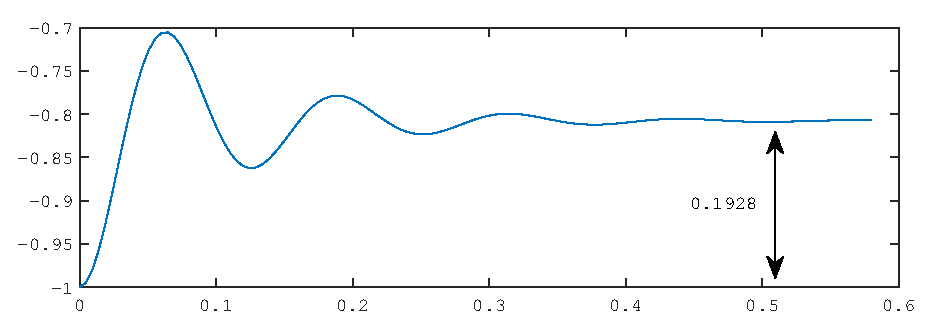
\includegraphics{images/Lab_1_SettlingTime_1.eps}%
  }\hfill
  \subfloat[Zoomed-in view on the settling behaviour of signal.%
  \label{fig:lab1:settling-time:b}]{%
    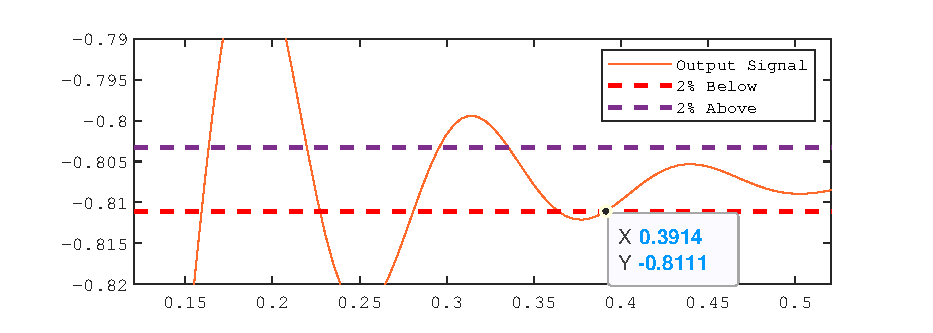
\includegraphics{images/Lab_1_SettlingTime_2.eps}%
  }
  \caption[Step Response for a Linear Plant depicting Settling Time Measurements]{
    The step response of some unknown plant with the \(2\%\)-settling time
    annotated in part (b). Observe how the the signal stays in
    the \(2\%\) region, demarcated by the broken lines,
    after the settling time of \(\SI{391.4}{ms}\) is attained.
  }
  \label{fig:lab1:settling-time}
\end{figure}
%
The settling time is a measure of long-term behaviour.
The notion is best depicted by Figure
\ref{fig:lab1:settling-time}.
In Figure~\ref{fig:lab1:settling-time:a} the ``net'' final value is
measured \emph{from the base to the top} of the signal. Then \(2\%\) of the
settling value is computed to define a cut-off point above and below the final
value, depicted as the broken lines in Figure
\ref{fig:lab1:settling-time:b}. Notice how the signal \emph{stays} in the
settling region after the settling time.
The next characteristic of the step response worthy of measurement is the
time constant. First let us define the standard first order form for a first
order transfer function.
%
\begin{definition}[]{Standard First-Order Form}
  The standard first order form for a strictly proper, first-order transfer
  function \(P(s)\) is
  \[
    P(s) = \frac{K}{\tau s + 1},
  \]
  where \(\tau, K \in \Real.\) The number \(\tau\) is called the \textbf{time
  constant}.
\end{definition}
%
It can be verified that the number \(K\) in the standard first order form
is simply the DC gain. The time constant can be estimated experimentally
in an easy way.
%
\begin{definition}[]{The Time Constant}
  For a first order plant \(P(s)\) and step input \(U(s) = \frac{1}{s},\)
  the time constant is the time \(\tau > 0\) it takes for
  the output \(y(t)\) to reach \(1-e^{-1} \approx 63\%\) of its final value.
\end{definition}
%
The time constant is a measure of transient, short-term behaviour. Note that,
unlike the settling time, the time constant only has meaning for a
first-order system. You will derive the relationship as one of your
deliverables.
%
\begin{procedure}[label={proc:lab1:p4}]
  In this procedure you will acquire the settling time and time constant
  of your plant \(P(s).\) First, \textbf{ensure} your plant is in open-loop
  configuration.
  \begin{enumerate}[label=(\arabic*)]
    \item{
      \textbf{Open} the signal generator block and \textbf{set} the type
      to be a square wave. Also, \textbf{set} the frequency to a low value,
      such as \(\SI{0.5}{Hz}.\) You will want to see atleast one step in
      the simulation but not too many more than that.
    }
    \item{
      \textbf{Run} the script \texttt{generate\_lab\_1\_plot.m} and inspect
      Figure 1, which depicts the input and output signal.
    }
    \item{
      Using cursors, \textbf{measure} the ``net'' final value by measuring from
      \emph{the base value of the signal to the final value}.
    }
    \item{
      Using the above measurement, \textbf{calculate} the \(63\%\) point
      where the time constant is found and \textbf{calculate} the \(2\%\)
      margins where the settling time is found.
    }
    \item{
      Using cursors, \textbf{measure} the time constant and settling times.
    }
  \end{enumerate}
\end{procedure}
%
\begin{deliverable}[label={lab1:d4}]
  \textbf{Capture the figure} you used to measure the settling time and
  time constant in Procedure~\ref{proc:lab1:p4}. \textbf{Show} your cursors.
\end{deliverable}
%
\begin{procedure}[label={proc:lab1:p5}]
  Repeat Procedure~\ref{proc:lab1:p4} for the closed-loop system described in
  Procedure~\ref{proc:lab1:p3}.
\end{procedure}
%
\begin{deliverable}[label={lab1:d5}]
  \textbf{Capture the figure} you used to measure the settling time and
  time constant in Procedure~\ref{proc:lab1:p5}. \textbf{Show} your cursors.
\end{deliverable}
%

\subsection{On Saturation or Clipping}
In practice, unlike in simulation, the signals we can apply to a system are
limited. This may be an inherent limitation, e.g.
power supply limitations, or a self-imposed safety limitation, e.g.
the angular velocity of an autonomous vehicle. Understanding where these hard
constraints appear in your control system is important, as usually these
constraints have \emph{nonlinear} effects! Ideally, we want to remain in
the region which has linear behaviour.

The only type of constraint you will encounter in these labs is the saturator
constraint. A \textbf{saturator}, or \textbf{clipper} as it is known in
electronics, limits a signal's maximum and minimum value to some preset
constant. In this section, you will attempt to find this limit.
%
\begin{procedure}[label={proc:lab1:p6}]
  \textbf{Put} your system in open-loop. \textbf{Set} the signal generator to
  generate a sinusoid with amplitude \(1\) at a low frequency.
  \textbf{Set} the gain \(K_p\) to \(1\) and \textbf{simulate}.
  \textbf{Increase} the gain \(K_p\) and \textbf{simulate} until you can
  observe the effects of saturation.
\end{procedure}
%
\begin{deliverable}[label={lab1:d6}]
  \textbf{Capture} the figure depicting the effects of saturation.
  \textbf{Record} the value of \(K_p\) where you had clipping occur.
\end{deliverable}

\section{Report Deliverable}
Good job! You made it through Lab 1. You are required to submit a report
that verifies you completed Lab 1 and that you understand the procedures you
performed. In addition to including
\begin{itemize}
  \item{Deliverable~\ref{lab1:d1},}
  \item{Deliverable~\ref{lab1:d2},}
  \item{Deliverable~\ref{lab1:d3},}
  \item{Deliverable~\ref{lab1:d4},}
  \item{Deliverable~\ref{lab1:d5} and}
  \item{Deliverable~\ref{lab1:d6}}
\end{itemize}
in your report,
you are required to answer the questions of the following deliverable.
Make sure to leverage your other deliverables in your answers!
\begin{deliverable}[label={lab1:report}]
  \begin{enumerate}[label={(\arabic*)}]
    \item{
      \label{lab1:report:q1}
      \textbf{Derive} a formula for the DC gain of \(P(s)\) in terms of
      \(a, b, T.\)
      \emph{Hint: Recall that the DC gain for a stable system \(G(s)\)
      is just \(G(0).\)}
    }
    \item{
      \label{lab1:report:q2}
      You know that your plant takes the form
      \[
        P(s) = \frac{b T}{s + a T}\quad ,
      \]
      for \(a, b > 0\) and \(T \in \{10, 100\}.\) \textbf{Derive} a
      formula for the bandwidth of \(P(s)\) in terms of \(a, b, T.\)
      \emph{Hint: Remember that the bandwidth frequency \(\omega\) solves
      the equation}
      \[
        \frac{\left\|P(j \omega)\right\|}{\left\|P(0)\right\|}
        =
        \frac{1}{\sqrt{2}}.
      \]
      \emph{Solve the expression for \(\omega.\) As
      an additional hint, you should get a polynomial in \(\omega^2\) which
      you can solve.}
    }
    \item{
      \label{lab1:report:q3}
      Using the formulas you derived in~\ref{lab1:report:q1} and
      \ref{lab1:report:q2} and the estimates of your bandwidth and DC gain
      in Procedures~\ref{proc:lab1:p1} and~\ref{proc:lab1:p2},
      \textbf{estimate} \(a, b, T.\) Recall that \(T\) can only take on
      values \(10\) or \(100.\)
    }
    \item{
      \label{lab1:report:q4}
      \textbf{Compare} the estimates of \(a, b, T\) made in
      \ref{lab1:report:q3} to your actual parameters.
      \textbf{Open} the ``\texttt{Lab\_1\_Data.sldd}'' to see your plant
      parameters. If there are discrepencies, explain why.
    }
    \item{
      \label{lab1:report:q5}
      \textbf{Find} a formula for the time constant of \(P(s)\) in terms of
      \(a, b, T.\) \emph{Hint: If you put \(P(s)\) in standard first order
      form, can you see what the time constant is?}
    }
    \item{
      \label{lab1:report:q6}
      \textbf{Find} the formula for the \(2\%\) settling time of \(P(s)\) in terms of \(a, b, T.\)
      \emph{Hint: You know \(P(s),\) the input \(U(s) = \frac{1}{s}\) and that
      the output is}
      \[
        Y(s) = P(s) U(s).
      \]
      \emph{Solve for an explicit expression for \(y(t)\) in the time domain.
      Then find how long it takes to reach \(2\%\) of the DC gain (the steady
      state value for a unit step)}
    }
    \item{
      \label{lab1:report:q7}
      Using the formulas you derived in~\ref{lab1:report:q5} and
      \ref{lab1:report:q6} and the estimates of your settling time and
      time constant in Procedure~\ref{proc:lab1:p4},
      \textbf{estimate} \(a, b, T.\)
    }
    \item{
      \label{lab1:report:q8}
      \textbf{Compare} the estimates of \(a, b, T\) made in
      \ref{lab1:report:q7} to your actual parameters.
    }
    \item{
      \label{lab1:report:q9}
      \textbf{Find} the transfer
      function from the input to the output when the system is in
      closed-loop, treating \(a, b, T, K_p\) as just unknown parameters.
      \emph{Hint: In closed loop you can write the input to the plant as
      \(U(s) = K_p(R(s) - Y(s))\)
      where \(R(s)\) is the input to the loop summing junction. See
      Figure~\ref{fig:lab1:closing-loop}. Combine this with \(Y(s) = P(s)U(s)\)
      and isolate \(Y(s)\) to get an expression \(Y(s) = G(s) R(s)\) where
      \(G(s)\) is some transfer function. Put \(G(s)\) in standard first order form.}
    }
    \item{
      \label{lab1:report:q10}
      \textbf{Discuss} how closing the loop, in Procedure
      \ref{proc:lab1:p3}, affected the bandwidth and DC gain.
      \textbf{Justify} your answer using the transfer function
      found in~\ref{lab1:report:q9}.
    }
    \item{
      \label{lab1:report:q11}
      \textbf{Discuss} how closing the loop, in Procedure
      \ref{proc:lab1:p5}, affected the settling time and time constant.
      \textbf{Justify} your answer using the transfer function
      found in~\ref{lab1:report:q9}.
    }
    \item{
      \label{lab1:report:q12}
      \textbf{Discuss} why we want to know the saturator limits. What would
      happen if we performed control design without verifying our control
      stayed within limits?
    }
  \end{enumerate}
\end{deliverable}

\subsection{Grading Scheme}
The grading scheme is shown in Table~\ref{tab:lab1:grading}. The breakdown of
your grade is shown per deliverable except in the case of the lab
questions where it is shown per question.
%
\begin{table}
\centering
\begin{tabular}{c|l|c}
        & Deliverable           & Marks  \\ \hline
        & \ref{lab1:d1}         & 2       \\ \hline
        & \ref{lab1:d2}         & 2       \\ \hline
        & \ref{lab1:d3}         & 2       \\ \hline
        & \ref{lab1:d4}         & 2       \\ \hline
        & \ref{lab1:d5}         & 2       \\ \hline
        & \ref{lab1:d6}         & 2       \\ \hhline{=|=|=}
Lab Subtotal&                       & 12      \\ \hhline{=|=|=}
        & \ref{lab1:report}~\ref{lab1:report:q1}  & 1       \\ \hline
        & \ref{lab1:report}~\ref{lab1:report:q2}  & 1       \\ \hline
        & \ref{lab1:report}~\ref{lab1:report:q3}  & 3       \\ \hline
        & \ref{lab1:report}~\ref{lab1:report:q4}  & 3       \\ \hline
        & \ref{lab1:report}~\ref{lab1:report:q5}  & 1       \\ \hline
        & \ref{lab1:report}~\ref{lab1:report:q6}  & 1       \\ \hline
        & \ref{lab1:report}~\ref{lab1:report:q7}  & 3       \\ \hline
        & \ref{lab1:report}~\ref{lab1:report:q8}  & 3       \\ \hline
        & \ref{lab1:report}~\ref{lab1:report:q9}  & 1       \\ \hline
        & \ref{lab1:report}~\ref{lab1:report:q10} & 5       \\ \hline
        & \ref{lab1:report}~\ref{lab1:report:q11} & 5       \\ \hline
        & \ref{lab1:report}~\ref{lab1:report:q12} & 1       \\ \hhline{=|=|=}
Report Subtotal&  & 28 \\ \hhline{=|=|=}
  Total &                       & 40
\end{tabular}
\caption[Grading Scheme for Lab 1]{Grading scheme for Lab 1.}
\label{tab:lab1:grading}
\end{table}
%

\chapter{Second-Order System Identification and Analysis}\label{Lab:2}
A large majority of systems we wish to control are physical systems. These
systems are often modelled using Newton's laws
\[
\begin{aligned}
  \mathrm{mass}~\frac{\mathrm d^2}{\mathrm{d}t^2}~\mathrm{position}
    &= \sum \mathrm{natural~forces} + \mathrm{applied~force},\\
  \mathrm{inertia}~\frac{\mathrm d^2}{\mathrm{d}t^2}~\mathrm{orientation}
    &= \sum \mathrm{natural~torques} + \mathrm{applied~torque},
\end{aligned}
\]
These systems --- when
they are linear --- result in second-order transfer functions from the
applied input (forces or torques) to the output (position and orientation).
It follows that if we want to understand how to effectively control physical
systems then we must first understand second-order systems and their
properties!

In this lab you will explore the generic characteristics of a second-order
linear system. You will discover the limitations of proportional error
feedback control --- the most na\'ive of control laws --- when applied to
a physical system. This motivates consideration of
more complicated control strategies. Labs 4 and 5 will explore these options.

\emph{A word of caution. This is the final lab where it is possible to
to find out the parameters of your system by inspecting the data file.
This, in principal, allows you to back-calculate what your procedures should
tell you. This was intentional to allow
you to check your work and ensure you understand how to perform the procedure.
However, future labs will assume you've perfected this procedure.
The parameters will be fairly well hidden like how it is sometimes in the
\texttt{\#RealWorld}. So, make sure you understand how to perform the
procedures!}

\section{Objectives}
The primary objectives of this lab are to
\begin{enumerate}[label=(\arabic*)]
  \item{
    \textbf{Learn} the characteristic properties of a standard second-order linear system.
  }
  \item{
    \textbf{Identify} the parameters of a standard second-order linear system.
  }
  \item{
    \textbf{Learn} how to acquire a Bode plot, the frequency response,
    and \textbf{understand} how to interpret it.
  }
  \item{
    \textbf{Explore} how a proportional control feedback affects the response
    of a second-order system.
  }
\end{enumerate}

\section{Experimental Procedure}
This entire lab will be done using the ``\texttt{Lab\_2.slx}'' Simulink model.
In there you will
find a number of blocks already placed for you in an open loop configuration:
\begin{itemize}
  \item{a step input,}
  \item{a summing junction,}
  \item{an adjustable gain block,}
  \item{a ``fill-in'', zero disturbance block,}
  \item{a ``plant'', the system we are going to analyze, and}
  \item{a terminator.}
\end{itemize}
This time we will \emph{not} use the signal generator and instead leverage
the Model Linearizer App. Its usage is described in Appendix
\ref{App:Simulink:ModelLinearizer}. You may acquire the step response
using the techniques described in Lab~\ref{Lab:1} but to acquire the frequency
response you will have to use the Model Linearizer app. In future, we will
primarily rely on the Model Linearizer app as it'll
unify all your data collection
requirements and is far easier to use than modifying a script and turning
on/off logging. For this lab, the input signal starts off configured
as \(r\) and the output signal as \(y.\) You will have to change it later
in the lab.
%
The plant --- labelled \(P(s)\) in the Simulink diagram --- can be assumed
to be a transfer function taking the form
\[
  P(s) = \frac{\hat{K}\omega_n^2}{s^2 + 2\zeta\omega_n s + \omega_n^2}.
\]
This form has a special name.
%
\begin{definition}[]{Standard Second-Order Form}
  The standard second-order order form for a strictly proper, second-order
  transfer function \(P(s)\) with no zero is
  \[
    P(s) = \frac{\hat{K} \omega^2}{s^2 + 2 \zeta \omega s + \omega^2}.
  \]
  where \(\omega\) is called the \textbf{natural frequency} and
  \(\zeta\) is the \textbf{damping ratio}.
\end{definition}
%
The primary goal of this experiment is to (1) estimate \(\zeta,\)\(\omega_n,\)
and \(\hat{K},\) (2) explore the characteristics of your system and
(3) see how the characteristics change under a proportional error controller.
When analyzing the \emph{closed loop system}, we put our system in the form
depicted by Figure~\ref{fig:lab2:closing-loop}.
%
\begin{figure}
  \centering
  \begin{tikzpicture}[x=1in, y=1in]
    \node [draw, block] (Controller) {\(K_p\)};
    \node [draw, block, right=0.5 of Controller] (Plant) {\(P(s)\)};
    \node [draw, summer, left=0.5 of Controller] (Sum) {};
    \node [draw, summer, right=0.5 of Plant] (DistSum) {};
    \node [above=0.5 of DistSum] (AboveDistSum) {};
    \node [below=0.5 of Sum] (BelowSum) {};

    \draw [arrow, signal]
      (AboveDistSum.base)
      --
      (DistSum.north)
      node [above right, annotate] {\(d\)};
    \draw [arrow, signal]
      (Controller.east) -- (Plant.west)
      node [below left, annotate] {\(u\)};
    \draw [arrow, signal]
      (Plant.east)
      --
      (DistSum.west)
      node [below left, annotate] {\(+\)};
    \draw [arrow, signal]
      (DistSum.east)
      --
      +(0.5, 0)
      |-
      (BelowSum.base)
      --
      (Sum.south)
      node [below right, annotate] {\(-\)};
    \draw [arrow, signal]
      (Sum.east) -- (Controller.west);
    \draw [arrow, signal]
      ($(Sum.west)+1*(-0.5, 0)$) -- (Sum.west)
      node [below left, annotate] {\(r\)};
    \draw [arrow, signal]
      (DistSum.east) -- +(1, 0)
      node [below, annotate] {\(y\)};
  \end{tikzpicture}
  \caption{
    Closing the loop around the Plant \(P(s)\) for Lab 2. Note that the
    loop is closed \emph{after} the disturbance has been added to the output.
  }
  \label{fig:lab2:closing-loop}
\end{figure}
%

\subsection{Measuring the Characteristics of a Second Order System}
In Lab~\ref{Lab:1}, you learned about the DC gain, the bandwidth, and
settling time of a first-order system.
We will use these characteristics, as well as one more new one, to help
characterize a second order plant.
%
Your deliverable for this section is
%
\begin{deliverable}[label={lab2:d1}]
  \textbf{Capture a figure} showing your system's open loop step response.
  \textbf{Measure} and \textbf{record}
  \begin{enumerate}[label=(\arabic*)]
    \item{the steady-state value \(y_{\mathrm{ss}},\)}
    \item{
      the time-to-peak value \(T_{\mathrm{peak}}\) and
      the peak value \(y_{\mathrm{max}},\) and
    }
    \item{
      the \(2\%\) settling time \(T_{\mathrm{s}}.\)
    }
  \end{enumerate}
  The figure included in your report must have \textbf{cursors} at the peak
  value and steady-state value.
\end{deliverable}
%
You are already familiar with most of these measurements. The new measurements
are the peak related measurements. For us, the following definition suffices.
%
\begin{definition}[]{Time-To-Peak and Overshoot}
  Let \(G(s)\) be a proper, stable transfer function
  that maps an input signal \(u(t)\) to an output \(y(t).\)
%
  Let \(u(t)\) be the (not necessarily unit) step function. The peak value
  of \(y(t)\) is the maximum value \(y(t)\) obtains, mathematically expressed
  by\footnote{normally \(\sup\) is used but this suffices for our purposes.}
  \[
    y_\mathrm{max} \defineas \max_{\tau \in \Real} \left| y(\tau) \right|
  \]
  and the time it obtains the peak value, known as \textbf{time-to-peak}
  is defined as
  \[
    T_\mathrm{peak} \defineas \argmax_{\tau \in \Real} \left| y(\tau) \right|.
  \]
  Then, if \(y_\mathrm{ss}\) is the steady-state value of \(y(t),\) the
  \textbf{percent overshoot} is defined as
  \[
    \%\mathrm{OS}
      \defineas
        \frac{%
          \left|
            \left|y_\mathrm{max}\right| - \left|y_\mathrm{ss}\right|
          \right|%
        }{%
          \left| y_\mathrm{ss}\right|%
        }.
  \]
\end{definition}
%
Figure~\ref{fig:lab2:peak} depicts the measurements you perform to acquire
the percent overshoot. You measure the maximum value of the output
signal and the steady-state value of the signal. Then you
compute the relative error between the maximum value and the settling value of
the output.
%
\begin{figure}
  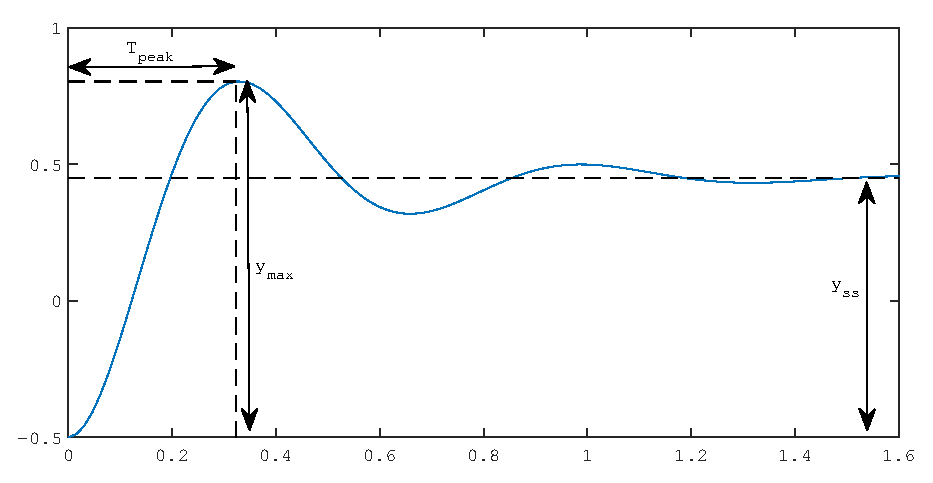
\includegraphics{images/Lab_2_Peak.eps}
  \caption[Depicting Overshoot Measurements for a Second-Order System.]{%
    The maximum peak occurs at time \(T_\mathrm{peak}\) with amplitude
    \(y_\mathrm{max}.\) The steady-state value is shown as \(y_{\mathrm{ss}}.\)
  }
  \label{fig:lab2:peak}
\end{figure}
%
\begin{procedure}[label={proc:lab2:p1}]
  In this procedure you will capture a variety of characteristics of
  your provided second-order system to achieve the goal of Deliverable
  \ref{lab2:d1} and to eventually characterize the parameters \(a,\)\(b\)
  and \(K.\)
  \begin{enumerate}[label=(\arabic*)]
    \item{
      \textbf{Ensure} your system is in the open loop configuration.
    }
    \item{
      \textbf{Ensure} that you indicate the signal before the summing junction
      is an input signal (Input Perturbation) and the signal after the plant
      is indicated as an output signal (Output Measurement). Refer
      to Appendix~\ref{App:Simulink:ModelLinearizer:2} for more information
      on how to do so.
    }
    \item{
      \textbf{Open} the Model Linearizer app and \textbf{capture} a
      step response. Refer to Appendix~\ref{App:Simulink:ModelLinearizer:3}
      on how to do so.
    }
    \item{
      \textbf{Measure} and \textbf{record} the following parameters of the
      output signal:
      \begin{itemize}
        \item{
          the steady-state value \(y_{\mathrm{ss}},\)
        }
        \item{
          the time-to-peak value \(T_{\mathrm{peak}}\) and
          the peak value \(y_{\mathrm{max}},\)
        }
        \item{
          the \(2\%\) settling time \(T_{\mathrm{s}}.\)
        }
      \end{itemize}
      \label{proc:lab2:p1:4}
    }
  \end{enumerate}
\end{procedure}

\subsection{Exploring Proportional Error Feeedback}
For this section you will explore how proportional error feedback affects
the behaviour of a second-order system. You will complete the following
deliverables.
%
\begin{deliverable}[label={lab2:d2}]
  \textbf{Capture} a single step response of your closed-loop system
  with a gain \(K_p \neq 1.\)
\end{deliverable}
%
\begin{deliverable}[label={lab2:d2b}]
  \textbf{Fill} three rows of the table
  \begin{center}
  \begin{tabular}{c|c|c|c|c}
    \(K_p\)
      & \(y_\mathrm{ss}\)
      & \(y_\mathrm{max}\)
      & \(T_\mathrm{peak}\)
      & \(\%\mathrm{OS}\) \\
    Gain
      & Steady-State Value
      & Peak Value
      & Time-To-Peak
      & Overshoot \\ \hline
    \(1\) & & & & \\ \hline
    Any & & & & \\ \hline
    Any & & & & \\ \hline
    & & & &
  \end{tabular}
  \end{center}
  for the closed loop system.
  Note that the overshoot is computed from \(y_\mathrm{ss}\) and
  \(y_\mathrm{max}.\)
\end{deliverable}

%
\begin{procedure}[label={proc:lab2:p2}]
  In this procedure you will explore a variety of gains \(K_p.\)
  \begin{enumerate}[label=(\arabic*)]
    \item{
      \textbf{Ensure} your system is in the closed-loop configuration
      as depicted in Figure~\ref{fig:lab2:closing-loop}.
    }
    \item{
      Choose a sequence of three gains to test. One of these gains
      must be \(K_p = 1.\) You may choose any value that is allowed by
      the slider gain provided to you in the Simulink Diagram.
    }
    \item{
      For each of your chosen gains \(K_p,\) \textbf{compute} the step
      response and \textbf{fill} the relevant row of the table
      in Deliverable~\ref{lab2:d2b}
    }
  \end{enumerate}
\end{procedure}

\subsection{Acquiring the Bandwidth in the Frequency-Domain}
Once again we will acquire the bandwidth of our system. We will do so for
\emph{both} the closed and open loop configurations. This time, however,
we will do so using the frequency response. In particular, you are asked
to complete the following deliverables.
%
\begin{deliverable}[label={lab2:d3a}]
  \textbf{Capture} a figure of the Bode plot for the open loop system.
  \textbf{Include} a cursor at the bandwidth frequency on the magnitude
  plot and a cursor where you estimated the DC gain.
\end{deliverable}
%
\begin{deliverable}[label={lab2:d3}]
  \textbf{Capture} a figure of the Bode plot for the closed loop system
  with unity gain (\(K_p = 1\)).
  \textbf{Include} a cursor at the bandwidth frequency on the magnitude
  plot.
\end{deliverable}
%
\begin{procedure}[label={proc:lab2:p3}]
  \begin{enumerate}[label=(\arabic*)]
    \item{
      \textbf{Ensure} your system is in the open-loop configuration.
      \textbf{Ensure} the gain \(K_p\) is set to \(1.\)
    }
    \item{
      \textbf{Open} the Model Linearizer App.
    }
    \item{
      \textbf{Acquire} a Bode plot. Your Bode plot will probably look a lot
      like Figure~\ref{fig:lab2:bode}. Note that, for some of you, you may
      have a little peak in the magnitude plot like in
      Figure~\ref{fig:lab2:bode:b}; this is normal!
      \label{proc:lab2:p3:3}
    }
    \item{
      \textbf{Measure} the DC gain on the Magnitude plot using a cursor.
      \emph{Recall: The DC gain is the value that the Magnitude Plot tends to
      as \(\omega \to 0.\)}
    }
    \item{
      \textbf{Measure} the frequency \(\omega\) at which the gain
      (magnitude plot) drops to a value \(\SI{3}{dB}\)
      below the DC gain measured in the previous step. This frequency
      is called the \textbf{bandwidth}.
      \label{proc:lab2:p3:5}
    }
  \end{enumerate}
\end{procedure}
%
\begin{procedure}[label={proc:lab2:p4}]
  \begin{enumerate}[label=(\arabic*)]
    \item{
      \textbf{Put} your system is in the closed-loop configuration as
      depicted by Figure~\ref{fig:lab2:closing-loop}.
      \textbf{Ensure} the gain \(K_p\) is set to \(1.\)
    }
    \item{
      Repeat steps~\ref{proc:lab2:p3:3}--\ref{proc:lab2:p3:5} of
      Procedure~\ref{proc:lab2:p3}.
      %\emph{Did you know you can overlay
      %this Bode plot on top of the Bode plot of Procedure~\ref{proc:lab2:p3}?
      %This is not required, but you can do so if you like.
      %To do so, take the Bode plot of the open loop system. Then, change the
      %configuration. Finally, instead of pressing ``\texttt{Bode Plot}'' press
      %a new button with the title of the plot. In my case it was
      %``\texttt{Bode Plot 1}.'' You will have something replicating that of
      %Figure~\ref{fig:lab2:bodeclosed}}
    }
  \end{enumerate}
\end{procedure}
%
\begin{figure}
  \centering
  \subfloat[A fairly well damped second order system.]{%
    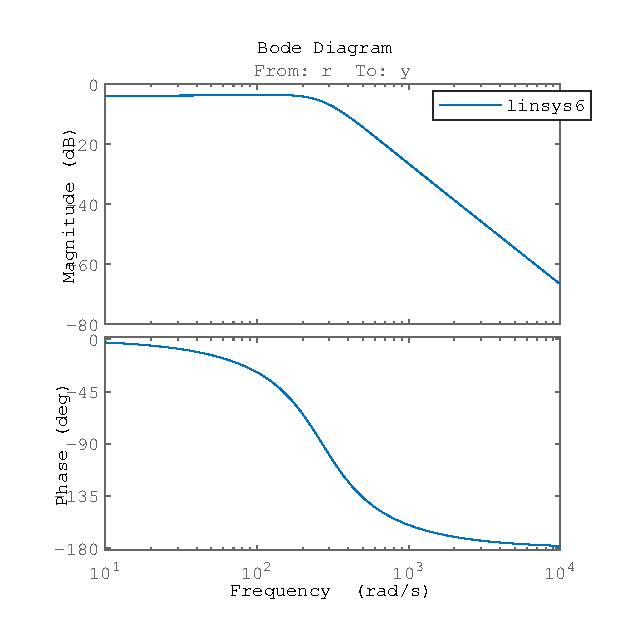
\includegraphics{images/Lab_2_Bode.eps}%
  }\hfill\\
  \subfloat[A much less damped, \(\zeta << 0.707,\) second order system.%
  \label{fig:lab2:bode:b}]{%
    \includegraphics{images/Lab_2_Bode_Peak.eps}%
  }\hfill\\
  \caption[Sample Bode Plots of a Second Order System]{
    Sample Bode plots of a second order system.
  }
  \label{fig:lab2:bode}
\end{figure}
%
% \begin{figure}
%   \centering
%   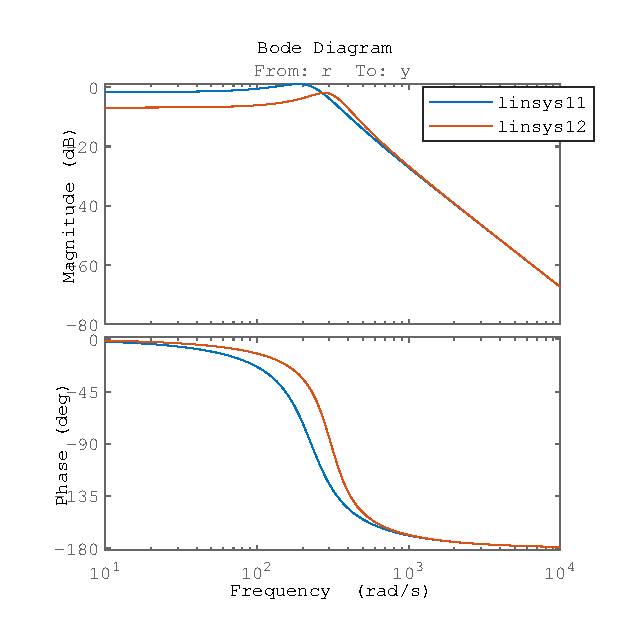
\includegraphics{images/Lab_2_Bode_ClosedLoop.eps}%
%   \caption[Sample Overlayed Bode Plots of a Second Order System]{
%     Sample overlayed Bode plots of a second order system.
%   }
%   \label{fig:lab2:bodeclosed}
% \end{figure}
%

\subsection{Disturbance Rejection}
You have almost completed the experimental part of this lab. This section
explores how the closed-loop affects disturbance rejection. Disturbances are
signals that we haven't modelled \emph{or} cannot be modelled and therefore
cannot account for. Naturally, large enough disturbances affect our ability to
control systems. The beauty of control is that we can design systems that
mitigate disturbances we do not explicitly model or know about! Here we will
find that our system can mitigate some types of disturbance signals, but not
all. The only deliverable for this section is
%
\begin{deliverable}[label={lab2:d4}]
  \textbf{Include} a Bode plot illustrating the response from the
  \emph{disturbance input signal} \(d(t)\) to the output signal \(y(t).\)
  \textbf{Include} a cursor on the magnitude plot at \emph{the bandwidth
  frequency of the closed loop system.} (The frequency found in
  Deliverable~\ref{lab2:d3})
\end{deliverable}
%
To fulfill this deliverable, you must acquire a Bode plot of the input to
output relationship between \(d\) and \(y.\)
%
\begin{procedure}[label={proc:lab2:p5}]
  For this procedure, you will change the input signal. You will remove the
  ``\texttt{Input Perturbation}'' annotation from the reference \(r\) and
  place it on the disturbance \(d.\)

  \begin{enumerate}[label=(\arabic*)]
    \item{
      \textbf{Ensure} the system is in the closed-loop configuration
      depicted in Figure~\ref{fig:lab2:closing-loop}.
      \textbf{Set} the gain \(K_p\) to \(1.\)
    }
    \item{
      \textbf{Remove} the ``\texttt{Input Perturbation}'' annotation from
      the reference signal. This amounts to repeating the process described
      in Appendix~\ref{App:Simulink:ModelLinearizer:2}, i.e. right click the
      signal wire \(r\) and press
      \texttt{Linear Analysis Points/Input Perturbation} so that the
      input perturbation icon disappears from the signal wire \(r.\)
    }
    \item{
      \textbf{Add} the ``\texttt{Input Perturbation}'' annotation to the
      the disturbance signal wire \(d.\)
    }
    \item{
      \textbf{Open} the Model Linearizer App and \textbf{acquire} a Bode
      plot. \emph{Expect the Bode plot to look substantially different than
      your previous Bode plots.}
    }
  \end{enumerate}
\end{procedure}

\section{Report Deliverable}
Good job! You made it through Lab~\ref{Lab:2}.
You are required to submit a report
that verifies you completed Lab~\ref{Lab:2} and that demonstrates you
understand the procedures you performed. In addition to including
\begin{itemize}
  \item{Deliverable~\ref{lab2:d1},}
  \item{Deliverable~\ref{lab2:d2},}
  \item{Deliverable~\ref{lab2:d2b},}
  \item{Deliverable~\ref{lab2:d3a},}
  \item{Deliverable~\ref{lab2:d3} and }
  \item{Deliverable~\ref{lab2:d4}}
\end{itemize}
in your report,
you are required to answer the questions of the following deliverable.
Make sure to leverage your other deliverables in your answers!
\begin{deliverable}[label={lab2:report}]
  \begin{enumerate}[label={(\arabic*)}]
    \item{
      Using the characteristics collected in Step~\ref{proc:lab2:p1:4} of
      Procedure~\ref{proc:lab2:p1}, \textbf{determine} the parameters
      \(\hat{K},\) \(\omega_n\) and \(\zeta\) that describe your plant \(P(s)\)
      in the standard second order form
      \[
        P(s) = \frac{\hat{K} \omega_n^2}{s^2 + 2 \zeta \omega_n s + \omega_n^2}
        .
      \]
      \emph{Notes: This time you drove the system with a unit
      step input. As a result, the steady-state value \(y_\mathrm{ss}\)
      is equal to the DC gain \(\hat{K}.\) The \(2\%\) settling time for a
      underdamped, standard second order system is approximated by the expression
      \[
        T_{2\%} \approx \frac{4}{\zeta \omega_n}
      \]
      and the percent overshoot is given by the formula
      \[
        \%\mathrm{OS} = 100 e^{\left(
          \frac{-\zeta \pi}{\sqrt{1-\zeta^2}}
        \right)}.
      \]
      So you should be able to solve for \(\hat{K}\) and \(\zeta\) first, then
      use them to solve for \(\omega_n.\)
      }
      \label{lab2:report:q1}
    }
    \item{
      It can be shown that the time-to-peak, another measurement you
      acquired, is equal to
      \[
        T_p = \frac{\pi}{\omega_n \sqrt{1-\zeta^2}}.
      \]
      Using your already acquired estimate of \(\zeta,\) \textbf{estimate}
      \(\omega_n\) using the time-to-peak.
      Based on your estimates, \textbf{explain} which you would rather use to
      estimate \(\omega_n:\) the time-to-peak or the \(2\%\) settling time.
      \label{lab2:report:q2}
    }
    \item{
      For the closed-loop diagram of Figure~\ref{fig:lab2:closing-loop},
      \textbf{compute} the transfer function from \(r\) to \(y.\)
      \textbf{Compute} the damping ratio, DC gain, and natural frequency of the
      closed-loop second-order system in terms of your plant's
      \(\hat{K},\) \(\omega_n\) and \(\zeta.\)
      \label{lab2:report:q3}
    }
    % \item{
    %   Given the open-loop damping ratio and natural frequency found in
    %   \ref{lab2:report:q1} and closed-loop damping ratio and natural
    %   frequency derived in~\ref{lab2:report:q2},
    %   \textbf{discuss} how closing the loop with unity feeback (\(K_p = 1\))
    %   affects the damping ratio and natural frequency of the
    %   second order system.
    %   \label{lab2:report:q3}
    % }
    \item{
      Using the table filled out in Deliverable~\ref{lab2:d2b} and the
      formulas you derived in~\ref{lab2:report:q2},
      \textbf{discuss} how changing the
      gain \(K_p\) affects the steady-state value \(y_\mathrm{ss},\) the
      time-to-peak \(T_p\) and the percent overshoot \(\%\mathrm{OS}.\)
      of the closed-loop second order step response.
      Also \textbf{discuss} how the settling time theoretically changes in the
      closed loop as a function of \(K_p\) using the estimate formula shown in
      \ref{lab2:report:q1}.
      \emph{\textbf{Ensure} you discuss every characteristic
      you've collected; if there is no trend, say so; if the trend is
      complicated (not simply linear in \(K_p\)), say so.}
      \label{lab2:report:q4}
    }
    \item{
      By leveraging your answer for~\ref{lab2:report:q4}, \textbf{explain} why
      proportional error feedback control is not sufficient to control a
      physical system.
      \label{lab2:report:q4b}
    }
    \item{
      Using the bandwidth frequencies found in Procedures~\ref{proc:lab2:p3}
      and~\ref{proc:lab2:p4}, \textbf{state} how closing the loop
      changed the bandwidth frequency.
      \label{lab2:report:q5}
    }
    % \item{
    %   \textbf{Why} is it desireable to be able to change the bandwidth
    %   of a system?
    %   \label{lab2:report:q7}
    % }
    \item{
      Leveraging Deliverable~\ref{lab2:d4}, \textbf{discuss} how well the
      closed loop system rejects disturbance signals.
      \emph{Your answer should depend on the disturbance input frequency
      \(\omega\) and the closed loop bandwidth frequency which you marked
      on your plot.}
      \label{lab2:report:q6}
    }
    % \item{
    %   For the open-loop configuration, \textbf{derive} the transfer function
    %   from the disturbance signal \(d\) to the output \(y.\)
    %   \textbf{Compare} the disturbance rejection properties between the
    %   open-loop and closed-loop system.
    %   \label{lab2:report:q7}
    % }
    \item{
      \textbf{Derive} the closed-loop transfer function from the
      disturbance \(d\) to the output \(y.\) How do the disturbance rejection
      properties change as you increase \(K_p\)? Do they improve or degrade?
      \emph{Hint: You should get a transfer function in the form
      \[
        \frac{s^2 + A s + B}{s^2 + A s + D}
      \]
      where \(A, B, D\) depend on the plant parameters and \(K_p.\)
      \(K_p\) should only appear in \(D.\) You can then split the
      above system into two subsystems
      \[
        \left[s^2 + A s + B\right]
        \left[\frac{1}{D}\frac{D}{s^2 + A s + D}\right]
      \]
      and recognize that \(K_p\) only affects the Bode plot of the latter
      system. This means it suffices to analyze the frequency response of
      \[
        \frac{1}{D}\frac{D}{s^2 + A s + D}
      \]
      as \(K_p\) varies. You can put this subsystem into standard second order
      form to aid in your analysis. You already should be able to argue how the
      DC gain and natural frequency of this new subsystem is affected by
      \(K_p,\) so it remains to connect this knowledge with how the Bode plot
      of this subsystem would be affected.
      }
      \label{lab2:report:q8}
    }
  \end{enumerate}
\end{deliverable}

\subsection{Grading Scheme}
The grading scheme is shown in Table~\ref{tab:lab2:grading}. The breakdown of
your grade is shown per deliverable except in the case of the lab
questions where it is shown per question.
%
\begin{table}
\centering
\begin{tabular}{c|l|c}
        & Deliverable           & Marks  \\ \hline
        & \ref{lab2:d1}         & 5       \\ \hline
        & \ref{lab2:d2}         & 5       \\ \hline
        & \ref{lab2:d3a}        & 5       \\ \hline
        & \ref{lab2:d3}         & 5       \\ \hline
        & \ref{lab2:d4}         & 5       \\ \hhline{=|=|=}
Lab Subtotal&                       & 25      \\ \hhline{=|=|=}
        & \ref{lab2:report}~\ref{lab2:report:q1}  & 3       \\ \hline
        & \ref{lab2:report}~\ref{lab2:report:q2}  & 2       \\ \hline
        & \ref{lab2:report}~\ref{lab2:report:q3}  & 3       \\ \hline
        & \ref{lab2:report}~\ref{lab2:report:q4}  & 4       \\ \hline
        & \ref{lab2:report}~\ref{lab2:report:q4b} & 1       \\ \hline
        & \ref{lab2:report}~\ref{lab2:report:q5}  & 1      \\ \hline
        & \ref{lab2:report}~\ref{lab2:report:q6}  & 3      \\ \hline
        & \ref{lab2:report}~\ref{lab2:report:q8}  & 4       \\ \hhline{=|=|=}
Report Subtotal&  & 21 \\ \hhline{=|=|=}
  Total &                       & 46
\end{tabular}
\caption[Grading Scheme for Lab 2]{Grading scheme for Lab 2.}
\label{tab:lab2:grading}
\end{table}
%

\chapter{Bringing it Together: Lateral Motion Control}\label{Lab:3}
Imagine you are a young, aspiring, junior engineer at VenX, a private company in an alternate Universe, manufucturing a mining probe on Venus.
\footnote{This society isn't particularly concerned about the environmental impact. It isn't our planet, right?}
Because of your junior status, they have only asked you to design a simple controller that ensures the lunar module lands at the correct location.
The controller you design controls the level of horizontal thrust to achieve a desired position relative to some point on the surface.
You may assume that all units are in standard units.
Distances are measured in meters, time is measured in seconds, mass is measured in kilograms and all other units are such that they are consistent with that.

\section{Objectives}
\begin{enumerate}[label=(\arabic*)]
  \item{
    \textbf{Use} the skills you learned in Labs~\ref{Lab:1} and~\ref{Lab:2}
    to identify parameters of an opaque, black box system.
  }
  \item{
    \textbf{Design} a proportional inner-loop controller that stabilizes the velocity and controls it to a desired value.
  }
  \item{
    \textbf{Design} a proportional outer-loop controller that stabilizes the relative position of the lunar module with respect to a set point on the ground.
  }
  \item{
    \textbf{Derive} a mathematical expression for your controller and use this to \textbf{achieve} a desired control objective.
  }
  \item{
    \textbf{Compare and contrast} your stabilizing control design with that of Lab~\ref{Lab:2}.
  }
  \item{
    \textbf{Appreciate} how your controller deals with disturbances and unmodelled dynamics.
  }
\end{enumerate}

\section{Experimental Procedure}\label{Lab:3:Experiment}
Unlike previous labs, you will now work with two Simulink models.
Moreover, this lab will involve a larger number of moving parts;
you will introduce three feedback interconnections!

In Section~\ref{Lab:3:Part:I} you will stabilize the physical plant that maps input forces to an output horizontal velocity.
You will treat velocity as the measurement (output).
You can then design a controller

\subsection{Part I: Stabilize and Identify the Plant}\label{Lab:3:Part:I}
Your deliverables for this subsection are
%
\begin{deliverable}[label={del:lab3:g1:1}]
  \textbf{Choose} and \textbf{record} a gain value \(K_1\) for your stabilizing gain.
\end{deliverable}
%
\begin{deliverable}[label={del:lab3:g1:2}]
   \textbf{Acquire} the step response from the signal labelled \(w(t)\) to the signal \(v(t)\) when the signal \(v(t)\) is connected to the \(G_1\) loop summing junction (aptly named ``\(G_1\) Loop'').
\end{deliverable}
%
\begin{deliverable}[label={del:lab3:g1:3}]
  \textbf{Measure} the time constant \(\tau_1\) of your stabilized plant using the step response acquired in Deliverable~\ref{del:lab3:g1:2}.
\end{deliverable}
%
This section concerns the Part I area of the Simulink model
\begin{center}
  \texttt{Lab\_3\_Velocity\_Controlled\_Landing\_Module.slx}.
\end{center}
In this lab, your plant is a simulated physical system.
The system has nonlinear dynamics, but we will treat it as a linear system and you will observe the power of linear control.
First, in order to even design a controller to achieve our objectives, we must stabilize the system.
The reason for this is quite simple. A physical system normally integrates the input force into velocity (and then position) and, unless there are external forces such as friction, the plant is of the form
\[
  P(s)
    =
      \frac{1}{M s}
\]
where \(M > 0\) is the mass of the landing module.
The step response of this system is unbounded.
It is true that there is friction in your model but it is often hard to model friction in reality, so we will take the above equation as our model.
To stabilize the plant, consider closing the loop in the following way
%
\begin{center}
  \begin{tikzpicture}[x=1in, y=1in]

    \node [draw, smooth_block] (Plant) {\(P(s)\)};
    \node [draw, smooth_block, left = 0.75 of Plant] (Gain1) {\(K_1\)};
    \node [draw, smooth_sum, left = 0.75 of Gain1] (Sum1) {};
    \node [right = 0.75 of Plant] (after_plant) {};
    \node [right = 0.75 of after_plant] (v) {};
    \node [left = 0.75 of Sum1] (w) {};

    \node [smooth_annotate, below = 0 of Gain1] {Stabilizing Gain};
    \node [smooth_annotate, below = 0 of Plant] {Plant};

    \draw [arrow, smooth_path]
      (Plant.east) -- (after_plant.base) -- (v.base);
    \draw [arrow, smooth_path]
      (Plant.east)
      --
      (after_plant.base)
      --
      +(0, -0.75)
      -|
      (Sum1.south)
      node [below right] {\(-\)};
    \draw [arrow, smooth_path]
      (Sum1.east)
      --
      (Gain1.west);
    \draw [arrow, smooth_path]
      (Gain1.east)
      --
      (Plant.west);
    \draw [arrow, smooth_path]
      (w.base)
      --
      (Sum1.west);
  \end{tikzpicture}
\end{center}
%
with a randomly chosen gain \(K_1 > 0.\)
The gain you choose is up to you but make sure you record it.
\begin{procedure}[label={proc:lab3:stabilize}]
  This procedure simply reiterates the steps above.
  \begin{enumerate}[label={(\arabic*)}]
    \item{%
      \textbf{Close} the loop as described above.
      You should connect the signal labelled \(v\) to the summing junction labelled ``\(G_1\) Loop.''%
    }
    \item{%
      \textbf{Choose} and \textbf{set} a random positive gain for \(K_1.\)
      The block is named ``Stabilizing Gain'' in the Simulink model.%
    }
    \item{%
      \textbf{Acquire} a step response from the signal \(w(t)\) to the signal \(v(t).\)
      Remember from Lab 2 that you need to set \(w\) as an input perturbation and \(v\) as an output measurement.
    }
    \item{%
      \textbf{Measure} the time constant of this system using the acquired step response. We will call this time constant \(\tau_1.\)
    }
  \end{enumerate}
\end{procedure}

\subsection{Part II: Reference Velocity Control Design}\label{Lab:3:Part:II}
When you performed Procedure~\ref{proc:lab3:stabilize}, you will have noticed that the step response was extremely slow.
In particular, you should notice that it took more than a minute of simulated time to achieve a speed of \SI{1}{m/s} (\SI{3.6}{km/h})!
If this is the response speed of our system, we will never be able to control it to a desired position.
In this section, you will solve this problem by designing a proportional error feedback controller that controls to a \emph{desired velocity} but with a much better time constant.
Your deliverables for this section are
%
\begin{deliverable}[label={del:lab3:g2:1}]
  \textbf{Acquire} a (unit) step response from the signal \(v_r(t)\) to the signal \(v(t).\)
  \textbf{Ensure} you have cursors that indicate the following:
  \begin{itemize}
    \item{the time constant is \(\frac{1}{\sqrt{50}} \approx 0.1414.\)}
    \item{the DC gain, or steady-state value, is \(1.\)}
  \end{itemize}
\end{deliverable}
%
This section concerns the Part II area of the Simulink model
\begin{center}
  \texttt{Lab\_3\_Velocity\_Controlled\_Landing\_Module.slx}.
\end{center}
The now stabilized plant, as a transfer function from \(w(t)\) to \(v(t),\) will be referred to as \(G_1(s)\) as is depicted below.
Verify for yourself that
\[
  G_1(s) = \frac{1}{\tau_1 s + 1}
\]
where \(\tau\) is the time constant of \(G_1(s)\) (as estimated in Deliverable~\ref{del:lab3:g1:timeconstant}).
Close the loop around \(G_1(s)\) with a proportional error feedback controller like so
%
\begin{center}
  \begin{tikzpicture}[x=1in, y=1in]

    \node [draw, smooth_block] (Plant) {\(P(s)\)};
    \node [draw, smooth_block, left = 0.25 of Plant] (Gain1) {\(K_1\)};
    \node [draw, smooth_sum, left = 0.25 of Gain1] (Sum1) {};
    \node [right = 0.25 of Plant] (after_plant) {};
    \node [right = 0.50 of after_plant] (v) {};
    \node [left = 0.50 of Sum1] (w) {};

    \draw [arrow, smooth_path]
      (Plant.east) -- (after_plant.base) -- (v.base)
      node [above right] {\(v(t)\)};
    \draw [arrow, smooth_path]
      (Plant.east)
      --
      (after_plant.base)
      --
      +(0, -0.50)
      -|
      (Sum1.south)
      node [below right] {\(-\)};
    \draw [arrow, smooth_path]
      (Sum1.east)
      --
      (Gain1.west);
    \draw [arrow, smooth_path]
      (Gain1.east)
      --
      (Plant.west);
    % \draw [arrow, smooth_path]
    %   (w.base)
    %   --
    %   (Sum1.west);

    \draw [smooth_area_path, fill = Blue, fill opacity = 0.50, text opacity = 1]
      ($(w)+(0.25, 0)$) -- +(0, 0.50) -| node[midway, above, color=Blue] {\(G_1(s)\)} ($(v)+(-0.50,0)$) -- +(0, -0.75) -| ($(w)+(0.25, 0)$);

    \node [draw, smooth_block, left = 0.25 of w] (Gain2) {\(K_2\)};
    \node [draw, smooth_sum, left = 0.50 of Gain2] (Sum2) {};
    \node [left = 0.50 of Sum2] (v_r) {};

    \draw [arrow, smooth_path]
      (Plant.east)
      --
      ($(v)+(-0.25,0)$)
      --
      +(0, -1)
      -|
      (Sum2.south)
      node [below right] {\(-\)};
    \draw [arrow, smooth_path]
      (Sum2.east)
      --
      (Gain2.west);
    \draw [arrow, smooth_path]
      (Gain2.east)
      --
      (Sum1.west);
    \draw [arrow, smooth_path]
      (v_r.base)
      --
      (Sum2.west)
      node [midway, above] {\(v_r(t)\)};

  \end{tikzpicture}
\end{center}
%
Verify that, when the loop is closed, the transfer function from \(v_r(t)\) to \(v(t),\) denoted as \(G_2(s)\) in the Simulink model, takes the form
\[
  G_2(s)
    = \frac{V(s)}{V_r(s)}
    = \frac{K_3 K_2}{1 + K_2} \frac{1}{\frac{\tau_1}{1 + K_2} s + 1}.
\]
%
\begin{procedure}[label={proc:lab3:speedup}]
  In this procedure you use another closed loop to accelerate the response of your system, thereby making it usable to do position step tracking.
  \begin{enumerate}[label={(\arabic*)}]
    \item{%
      \textbf{Close} the loop as described above.
      You should connect the signal labelled \(v\) to the summing junction labelled ``\(G_2\) Loop.''%
    }
    \item{%
      We would like to have the transfer function \(G_2(s)\) to have a time constant of \(\frac{1}{\sqrt{50}}.\)
      This would mean that, for a step change in the \emph{reference velocity}, the \emph{actual velocity} will reach \(63.3\%\) of the reference velocity in \SI{0.1414}{s}.
      Recognize that the time constant of this new closed loop system is
      \[
        \frac{\tau_1}{1 + K_2}
      \]
      where \(\tau_1\) is the time constant of \(G_1(s)\) that you measured earlier.
      As a result, \textbf{solve} for the \(K_2\) you need to have this time constant equal to \(\frac{1}{\sqrt{50}}.\)%
    }
    \item{%
      \textbf{Solve} for the gain \(K_3\) that ensures \(G_2(s)\) has a DC gain of \(1.\)%
    }
    \item{%
      \textbf{Set} the respective blocks corresponding to \(K_2\) and \(K_3\) in the Simulink diagram.%
    }
    \item{%
      \textbf{Acquire} the step response from the signal \(v_r(t)\) to the signal \(v(t).\)
      Remember again to change which signal is the input perturbation from Part I.%
    }
    \item{%
      \textbf{Place} cursors on the time constant and steady-state value to prove you met the specification.%
    }
  \end{enumerate}
\end{procedure}

\subsection{Part III: Reference Position Control Design}\label{Lab:3:Part:III}
Your deliverables for this part are
%
\begin{deliverable}[label={del:lab3:g3:1}]
   \textbf{Acquire} the step response from the signal labelled \(r(t)\) to the signal \(x(t)\) when the signal \(x(t)\) is connected to the \(G_3\) loop summing junction (aptly named ``\(G_3\) Loop'').
   This is the step response of the transfer function \(G_3(s)\) depicted in the Simulink model.
\end{deliverable}
%
\begin{deliverable}[label={del:lab3:g3:2}]
   \textbf{Run} the ``\texttt{visualize\_landing.m}'' script and \textbf{save} both Figures that are generated.
\end{deliverable}
%
This section concerns the Part III area of the Simulink model
\begin{center}
  \texttt{Lab\_3\_Position\_Controlled\_Landing\_Module.slx}.
\end{center}
You will notice that the other Simulink model you worked with is labelled \(G_2(s)\) in this model.
Since you have designed a controller that achieves a desired reference velocity, we leverage it in this model to design an outer loop controller that achieves a desired position.
Close the loop to arrive at a diagram
%
\begin{center}
  \begin{tikzpicture}[x=1in, y=1in]

    \node [draw, smooth_block] (G2) {\(G_2(s)\)};
    \node [draw, smooth_block, right = 0.75 of G2] (Int) {\(\frac{1}{s}\)};
    \node [draw, smooth_block, left = 0.75 of G2] (Gain4) {\(K_4\)};
    \node [draw, smooth_sum, left = 0.75 of Gain4] (Sum3) {};
    \node [right = 0.25 of Int] (after_int) {};
    \node [right = 0.50 of after_int] (x) {};
    \node [left = 0.50 of Sum3] (r) {};

    \draw [arrow, smooth_path]
      (G2.east) -- (Int.west)
      node [above, midway] {\(v(t)\)};
    \draw [arrow, smooth_path]
      (Int.east) -- (after_int.base) -- (x.base)
      node [above] {\(x(t)\)};
    \draw [arrow, smooth_path]
      (Int.east)
      --
      (after_int.base)
      --
      +(0, -0.50)
      -|
      (Sum3.south)
      node [below right] {\(-\)};
    \draw [arrow, smooth_path]
      (Sum3.east)
      --
      (Gain4.west);
    \draw [arrow, smooth_path]
      (Gain4.east)
      --
      (G2.west);
    % \draw [arrow, smooth_path]
    %   (w.base)
    %   --
    %   (Sum1.west);

    \draw [arrow, smooth_path]
      (r.base)
      --
      (Sum3.west)
      node [midway, above] {\(r(t)\)};

  \end{tikzpicture}
\end{center}
%
If you performed Part II correctly, the transfer function \(G_2(s)\) takes the
form
\[
  G_2(s) = \frac{1}{\frac{1}{\sqrt{50}}s + 1}.
\]
Verify that the transfer function from \(r(t)\) to \(x(t),\) denoted \(G_3(s)\) in the Simulink model, equals
\[
  G_3(s) = \frac{K_4\sqrt{50}}{s^2 + \sqrt{50} s + K_4 \sqrt{50}}.
\]
%
\begin{procedure}[label={proc:lab3:regulate}]
  You will make a specific choice for \(K_4\) in this procedure and then simulate the entire non-linear system.
  \begin{enumerate}[label={(\arabic*)}]
    \item{%
      \textbf{Close} the loop as described above.
      You should connect the signal \(x(t)\) to the \(G_3\) loop summing junction (aptly named ``\(G_3\) loop'').%
    }
    \item{%
      \textbf{Determine} and \textbf{set} the gain \(K_4\) so that the system \(G_3(s)\) is critically damped.
      To be clear, with your choice of \(K_4\) you should find that \(\zeta = 1\) when \(G_3(s)\) is put in standard form.%
    }
    \item{%
      \textbf{Acquire} the (unit) step response from the signal \(r(t)\) to the signal \(x(t).\)
      Remember to go into the other model file and remove any annotations you have used there before setting new ones in this model file.%
    }
    \item{%
      \textbf{Run} the ``\texttt{visualize\_landing.m}'' script and \textbf{save} both Figures that are generated.%
      \emph{Do not be alarmed that the behaviour does not look like the step response. You will be expected to address this discrepancy in your report.}
    }
  \end{enumerate}
\end{procedure}
%

\section{Report Deliverable}
Wow you made it through the Lab 3 experiment! Good job! As usual, you are expected to submit a report demonstrating that you completed the lab and that you understand the tasks performed.
In addition to including
\begin{itemize}
  \item{Deliverable~\ref{del:lab3:g1:1},}
  \item{Deliverable~\ref{del:lab3:g1:2},}
  \item{Deliverable~\ref{del:lab3:g1:3},}
  \item{Deliverable~\ref{del:lab3:g2:1},}
  \item{Deliverable~\ref{del:lab3:g3:1} and}
  \item{Deliverable~\ref{del:lab3:g3:2}}
\end{itemize}
in your report, you are required to answer the questions of the following deliverable.
Make sure to leverage your other deliverables in your answers!
\begin{deliverable}[label={lab3:report}]
  \begin{enumerate}[label={(\arabic*)}]
    \item{

    }
  \end{enumerate}
\end{deliverable}

\subsection{Grading Scheme}
The grading scheme is shown in Table~\ref{tab:lab3:grading}. The breakdown of
your grade is shown per deliverable except in the case of the lab
questions where it is shown per question.
%
\begin{table}
\centering
\begin{tabular}{c|l|c}
        & Deliverable           & Marks  \\ \hline
        & \ref{del:lab3:g1:1}         & 5       \\ \hline
        & \ref{del:lab3:g1:2}         & 5       \\ \hline
        & \ref{del:lab3:g1:3}        & 5       \\ \hline
        & \ref{del:lab3:g2:1}        & 5       \\ \hline
        & \ref{del:lab3:g3:1}         & 5       \\ \hline
        & \ref{del:lab3:g3:2}         & 5       \\ \hhline{=|=|=}
Lab Subtotal&                       & 25      \\ \hhline{=|=|=}
        & \ref{lab3:report}~\ref{lab2:report:q1}  & 3       \\ \hline
        & \ref{lab3:report}~\ref{lab2:report:q2}  & 2       \\ \hline
        & \ref{lab3:report}~\ref{lab2:report:q3}  & 3       \\ \hline
        & \ref{lab3:report}~\ref{lab2:report:q4}  & 4       \\ \hline
        & \ref{lab3:report}~\ref{lab2:report:q4b} & 1       \\ \hline
        & \ref{lab3:report}~\ref{lab2:report:q5}  & 1      \\ \hline
        & \ref{lab3:report}~\ref{lab2:report:q6}  & 3      \\ \hline
        & \ref{lab3:report}~\ref{lab2:report:q8}  & 4       \\ \hhline{=|=|=}
Report Subtotal&  & 21 \\ \hhline{=|=|=}
  Total &                       & 46
\end{tabular}
\caption[Grading Scheme for Lab 3]{Grading scheme for Lab 3.}
\label{tab:lab2:grading}
\end{table}
%

\chapter{PID Analysis}\label{Lab:4}
You are now a slightly more experienced junior engineer at VenX.
This time, you are designing an unmanned aerial vehicle that is dropped into the atmosphere and performs powered glides along predefined paths over the surface.
%
\begin{center}
  %\centering
  \input{Lab_4_UAV_PF.pdf_tex}%
  %\caption{Unmanned Aerial Vehicle (UAV) moving with respect to some line.}
  %\label{fig:lab4:uav}
\end{center}
%
The purpose is to do surveillance\footnote{Don't worry. The CEO of VenX, Lone Dusk, has assured you that the FBI are not using your technology for surveilling citizens in protests. Should you trust him? Probably not. But in this lab, you live in a utopia where people and the government are very honourable.} of the planet's surface to map out the landscape.

The controller you design controls the turning rate (\SI{}{rad/s}) and the output you measure is the distance to the straight line path \(y(t)\) (\SI{}{m}).
In practice the transfer function from this input to \(y(t)\) is highly nonlinear, but the senior engineers have designed an inner loop controller that makes the plant \(P(s)\) look like
\[
  P(s) = \frac{1}{s^2}.
\]
Take \texttt{ECE 486}\footnote{In the robotics course you will learn to just cancel the nonlinearities out.} if you are interested in how to do this.

\section{Objectives}\label{Lab:4:Objectives}
This goals of this lab are to
\begin{enumerate}[label=(\arabic*)]
  \item{
    \textbf{Learn} how the derivative and integral terms of a PID controller affect performance (desireably and undesireably).
  }
  \item{
    \textbf{Tune} a proportional-integral-derivative (PID) controller.
  }
  \item{
    \textbf{Learn} how to use the root locus to assist in control design.
  }
  \item{
    \textbf{Recognize} how zero dynamics can be introduced by controllers and how they can severely impact performance and analysis.
  }
\end{enumerate}
The deliverable dependency graph is
\begin{center}
\begin{tikzpicture}[x=1em, y=1em]
  \node[deliverable] (D1) {Deliverable\\\ref{del:lab4:p1:1}};
  \node[deliverable, below = 2 of D1] (D2) {Deliverable\\\ref{del:lab4:p2:1}--\ref{del:lab4:p2:3}};
  \node[deliverable, below = 2 of D2] (D3) {Deliverable\\\ref{del:lab4:p3:1}--\ref{del:lab4:p3:3}};
  \node[deliverable, right = 2 of D3] (Q1) {Deliverable\\\ref{lab4:report}~\ref{lab4:report:q1}--\ref{lab4:report:q2}};
  \node[deliverable, below = 2 of Q1] (Q4) {Deliverable\\\ref{lab4:report}~\ref{lab4:report:q4}};
  \node[deliverable, right = 2 of Q4] (Q5) {Deliverable\\\ref{lab4:report}~\ref{lab4:report:q5}};
  \node[deliverable, at = {(Q5|-D1)}] (Q3) {Deliverable\\\ref{lab4:report}~\ref{lab4:report:q3}};
  \node[deliverable, right = 2 of Q5] (Q6) {Deliverable\\\ref{lab4:report}~\ref{lab4:report:q6}};
  \node[deliverable, left = 2 of D3] (Q7) {Deliverable\\\ref{lab4:report}~\ref{lab4:report:q7}};

  \draw[signal, arrow] (D1.south) -- (D2.north);
  \draw[signal, arrow] (D2.south) -- (D3.north);
  \draw[signal, arrow] (D3.east) -- (Q1.west);
  \draw[signal, arrow] (D3.south) |- (Q4.west);
  \draw[signal, arrow] (Q4.east) -- (Q5.west);
  \draw[signal, arrow] (Q3.south) -- (Q5.north);
  \draw[signal, arrow] (Q5.east) -- (Q6.west);
  \draw[signal, arrow] (D3.west) -- (Q7.east);

\end{tikzpicture}
\end{center}

\section{Experimental Procedure}\label{Lab:4:Experiment}
This lab is split into three parts.
There is only one Simulink model.
In Part I you will analyze how the derivative term affects the stability of your system.
In Part II you will analyze how the integral term affects the performance of your system.
Finally in Part III you make an incremental change to your PID controller to improve your system's performance qualitatively.
The plant for this lab will be
\[
  P(s) = \frac{1}{s^2}.
\]

\subsection{Part I: The Proportional Derivative (PD) Controller}
The closed loop system under PD control takes the form
%
\begin{center}
  \begin{tikzpicture}[x=1in, y=1in]

    \node [draw, smooth_block] (Plant) {\(\frac{1}{s^2}\)};
    \node [draw, smooth_block, left = 0.50 of Plant] (Gain1) {\(K_d s + K_p\)};
    \node [draw, smooth_sum, left = 0.50 of Gain1] (Sum1) {};
    \node [right = 0.50 of Plant] (after_plant) {};
    \node [right = 0.50 of after_plant] (y) {};
    \node [left = 0.50 of Sum1] (r) {};

    \node [smooth_annotate, below = 0 of Gain1] {Controller};
    \node [smooth_annotate, below = 0 of Plant] {Plant};

    \draw [arrow, smooth_path]
      (Plant.east) -- (after_plant.base) -- (y.base) node [below right] {\(y\)};
    \draw [arrow, smooth_path]
      (Plant.east)
      --
      (after_plant.base)
      --
      +(0, -0.75)
      -|
      (Sum1.south)
      node [below right] {\(-\)};
    \draw [arrow, smooth_path]
      (Sum1.east)
      --
      (Gain1.west);
    \draw [arrow, smooth_path]
      (Gain1.east)
      --
      (Plant.west)
      node [below left] {\(u\)};
    \draw [arrow, smooth_path]
      (r.base)
      node [below left] {\(r\)}
      --
      (Sum1.west);
  \end{tikzpicture}
\end{center}
If you compute the closed loop transfer function \(G(s)\) from \(r(t)\) to \(y(t)\) you will find
\[
  G(s) = \frac{K_d s + K_p}{s^2 + K_d s + K_p}.
\]
As long as \(K_p, K_d > 0\) the closed loop system is stable.
Note that we have a zero appearing in the transfer function.
Assuming that the zero dynamics are fast, i.e. \(K_p \gg K_d,\) we can approximate the system by the transfer function
\[
  \tilde{G}(s) = \frac{K_p}{s^2 + K_d s + K_p}.
\]
It then should not surprise you that the intuition used for designing the gains in Lab~\ref{Lab:2} apply somewhat to the gains \(K_p\) and \(K_d.\)
You can see that decreasing (increasing) \(K_d\) while fixing \(K_p\) will result in a larger (smaller) settling time and larger (smaller) overshoot.
Decreasing (increasing) \(K_p\) while fixing \(K_d\) will result in smaller (larger) overshoot.
Of course, a real PID controller also has a non-zero integrator which can, at times, throw a wrench in this sort of analysis.
Your deliverable for this section is to
%
\begin{deliverable}[label={del:lab4:p1:1}]
  \textbf{Choose} and \textbf{record} a pair of gains \(K_p\) and \(K_d.\)
\end{deliverable}
%
and next procedure describes how to go about this.
%
\begin{procedure}[label={proc:lab4:kpkd}]
  In this procedure you will determine a pair \(K_p\) and \(K_d.\)
  \begin{enumerate}[label={(\arabic*)}]
    \item{%
      \textbf{Ensure} the loop of the Simulink model is closed as in the block diagram above.
    }
    \item{%
      \textbf{Pick} a random \(K_p\) and \(K_d\) in the slider range given in the Simulink model.
      \label{proc:lab4:kpkd:2}
    }
    \item{%
      \textbf{Run} the ``visualize\_uav.m'' MATLAB script and \textbf{inspect} Figure 2.
      If there are persistent oscillations in your response or if they don't dissipate around \SI{30}{s}, \textbf{repeat} step~\ref{proc:lab4:kpkd:2} with a different choice.
      Use your understanding of Lab~\ref{Lab:3} to motivate whether you should increase or decrease \(K_d\) or \(K_p.\)
    }
    \item{%
      Once you have settled on a choice for \(K_p\) and \(K_d,\)
      \textbf{run} the ``visualize\_uav.m'' MATLAB script and \textbf{inspect} Figure 2.
      \textbf{Observe} that there is a constant steady-state error.
    }
  \end{enumerate}
\end{procedure}

\subsection{Part II: Introducing an Integral Component}
We would like to eliminate the observed constant steady-state error.
How do we do this?
First we must determine why this error appears.
It is fair to ask:
``If our plant already has an integrator, how is it that there is constant steady-state error?''
In this simulation there is a constant \emph{input} disturbance similar to the \(d(t)\) of Lab~\ref{Lab:3}.
As you verified in Lab~\ref{Lab:3}, even an integrator in the plant cannot perfectly reject this input disturbance and can only attenuate it under proportional error feedback.
If we introduce a pole at the origin, i.e. an integrator, in the controller we can perfectly reject this error.
Unfortunately, there is a constraint on how large the integrator term can be.
Your deliverable for this part is to simply choose an integrator gain.
%
\begin{deliverable}[label={del:lab4:p2:1}]
  \textbf{Choose} and \textbf{record} a gain \(K_i > 0\) that perfectly rejects the step disturbance while ensuring closed loop stability.
\end{deliverable}
%
To do this we will make use of the root locus method.
As such, you are required to also produce a relevant root locus.
%
\begin{deliverable}[label={del:lab4:p2:2}]
  \textbf{Acquire} the root locus generated by the ``part\_2.m'' MATLAB script.
  \textbf{Place} a cursor on a point where the system is unstable so that you recognize how large \(K_i\) is allowed to be.
  \textbf{Save} the figure.
\end{deliverable}
%
Finally you will acquire the complete system response.
%
\begin{deliverable}[label={del:lab4:p2:3}]
  \textbf{Acquire} Figure 2 by running the ``visualize\_uav.m'' MATLAB script and \textbf{save} it.
\end{deliverable}
%
Your complete PID control system looks like
%
\begin{center}
  \begin{tikzpicture}[x=1in, y=1in]

    \node [draw, smooth_block] (Plant) {%
      \(\frac{1}{s^2}\)%
    };
    \node [draw, smooth_sum, left = 0.25 of Plant] (Sum2) {};
    \node [draw, smooth_block, left = 0.25 of Sum2] (Gain1) {%
      \(K_p + K_d s\)%
    };
    \node [draw, smooth_block, above = 0.25 of Gain1] (Gain2) {%
      \(\frac{K_i}{s}\)%
    };
    \node [draw, smooth_sum, left = 0.50 of Gain1] (Sum1) {};
    \node [right = 0.75 of Plant] (after_plant) {};
    \node [right = 0.75 of after_plant] (y) {};
    \node [left = 0.75 of Sum1] (r) {};

    \draw [arrow, smooth_path]
      (Plant.east) -- (after_plant.base) -- (y.base) node [below right] {\(y\)};
    \draw [arrow, smooth_path]
      (Plant.east)
      --
      (after_plant.base)
      --
      +(0, -0.75)
      -|
      (Sum1.south)
      node [below right] {\(-\)};
    \draw [arrow, smooth_path]
      (Sum1.east)
      --
      (Gain1.west);
    \draw [arrow, smooth_path]
      (Sum1.east)
      --
      +(0.25, 0)
      |-
      (Gain2.west);
    \draw [arrow, smooth_path]
      (Gain1.east)
      --
      (Sum2.west);
    \draw [arrow, smooth_path]
      (Gain2.east)
      -|
      (Sum2.north);
    \draw [arrow, smooth_path]
      (Sum2.east)
      --
      (Plant.west)
      node [below left] {\(u\)};
    \draw [arrow, smooth_path]
      (r.base)
      node [below left] {\(r\)}
      --
      (Sum1.west);
  \end{tikzpicture}
\end{center}
%
where you have determined \(K_p\) and \(K_d\) already.
The closed loop poles of this system\footnote{Notice what I do not say. I am \textbf{not} saying the closed loop zeros or the DC gain are the same.} are the same as the poles of the closed loop system
%
\begin{center}
  \begin{tikzpicture}[x=1in, y=1in]

    \node [draw, smooth_block] (Plant) {%
      \(\frac{1}{s(s^2 + K_d s + K_p)}\)%
    };
    \node [draw, smooth_block, left = 0.50 of Plant] (Gain1) {%
      \(K_i\)%
    };
    \node [draw, smooth_sum, left = 0.50 of Gain1] (Sum1) {};
    \node [right = 0.50 of Plant] (after_plant) {};
    \node [right = 0.50 of after_plant] (y) {};
    \node [left = 0.50 of Sum1] (r) {};

    \draw [arrow, smooth_path]
      (Plant.east) -- (after_plant.base) -- (y.base);
    \draw [arrow, smooth_path]
      (Plant.east)
      --
      (after_plant.base)
      --
      +(0, -0.50)
      -|
      (Sum1.south)
      node [below right] {\(-\)};
    \draw [arrow, smooth_path]
      (Sum1.east)
      --
      (Gain1.west);
    \draw [arrow, smooth_path]
      (Gain1.east)
      --
      (Plant.west);
    \draw [arrow, smooth_path]
      (r.base)
      --
      (Sum1.west);
  \end{tikzpicture}
\end{center}
It follows that if we plot the (positive gain) root locus of \(\frac{1}{s(s^2 + K_d s + K_p)}\) and choose a gain so that the poles of this system meet our desired specifications, we can use this very same gain as \(K_i\) in our closed loop system to produce the same poles that meet the same specifications.
The next procedure guides you through these steps.
%
\begin{procedure}[label={proc:lab4:ki}]
  In this procedure you will produce a root locus and make an initial choice for the gain \(K_i.\)
  \begin{enumerate}[label={(\arabic*)}]
    \item{%
      \textbf{Run} the ``part\_2.m'' MATLAB script with the variables \texttt{Kp} and \texttt{Kd} set to your chosen gains from Part I and \textbf{inspect} Figure 3.
    }
    \item{%
      \textbf{Observe} that if \(K_i\) is too large, the system will be rendered unstable. \textbf{Place a cursor} on one such point on the root locus.
      \textbf{Save} this Figure for Deliverable~\ref{del:lab4:p2:2}.
    }
    \item{%
      \textbf{Take note} of the gain depicted by your cursor in the previous step.
      If \(K_i\) takes on a value larger than this gain, your system may be rendered unstable!
    }
    \item{%
      \textbf{Pick any} value of \(K_i\) between \(0\) and the maximum gain defined by the previous step.
    }
    \item{%
      \textbf{Read} the cursor to find out what the gain value is.
      \textbf{Record} this gain value as the value you choose for \(K_i\) producing Deliverable~\ref{del:lab4:p2:1}.
    }
  \end{enumerate}
\end{procedure}
%
Now that you have chosen \(K_i\) you are ready to test out whether it worked.
There is no deliverable for the next procedure as it is only a verification that the previous procedures went smoothly.
%
\begin{procedure}[label={proc:lab4:verify}]
  You will now verify your choice of \(K_i.\)
  \begin{enumerate}[label={(\arabic*)}]
    \item{%
      \textbf{Set} the integrator gain with your chosen value of \(K_i.\)
    }
    \item{%
      \textbf{Run} the ``visualize\_uav.m'' MATLAB script and \textbf{inspect} Figures 1 and 2.
      \textbf{Observe} that the UAV continues to track the path but now does so without steady-state error.
      \textbf{Save} Figure 2 for Deliverable~\ref{del:lab4:p2:3}.
    }
  \end{enumerate}
\end{procedure}

\subsection{Part III: Tune your Controller}
Now that we have eliminated the steady-state error, you may observe more extreme oscillations or a large overshoot.
In this part, you will make an attempt to improve the performance of your controller.
Your deliverable for this section is
%
\begin{deliverable}[label={del:lab4:p3:1}]
  \textbf{Acquire} the root locus plots generated by the ``part\_3.m'' MATLAB script with your PID gains determined at the end of Part II.
  \textbf{Save} the figures.
\end{deliverable}
%
and you will use this information, alongside your other intuitions, to guide another choice of gains.
%
\begin{deliverable}[label={del:lab4:p3:2}]
  \textbf{Determine} a new set of gains \(K_p,\) \(K_i\) and \(K_d\) that in some way improve the performance of your UAV.
  This may be in reduced overshoot, or reduced settling time, for example.
  You may consider any characteristic you consider undesireable.
\end{deliverable}
%
Finally, you will acquire and save Figure 2 generated by ``visualize\_uav.m'' to prove you have achieved perfect tracking.
%
\begin{deliverable}[label={del:lab4:p3:3}]
  \textbf{Acquire} Figure 2 by running the ``visualize\_uav.m'' MATLAB script and \textbf{save} it to depict the improved performance.
  If there is no improvement, \textbf{acquire} atleast three simulations (of three different gain choices) producing Figure 2 and \textbf{save all of them}. \textbf{Record} the changes you made.
\end{deliverable}
%
\begin{procedure}[label={proc:lab4:tune}]
  There is no explicit procedure to tune your controller but this high-level series of steps can help you make your initial changes.
  \begin{enumerate}[label={(\arabic*)}]
    \item{%
      \textbf{Run} the ``part\_3.m'' MATLAB script with the variables \texttt{Kp}, \texttt{Kd} and \texttt{Ki} set to your gains determined in Part II.
      \textbf{Save} the figures (4, 5, 6) for Deliverable~\ref{del:lab4:p3:1}.
    }
    \item{%
      \textbf{Inspect} the root locus plots generated.
      Each root locus depicts your current closed loop poles with filled black circles.
      You can therefore see how changing any gain would change the location of the closed loop poles and thereby change the behaviour of your final closed loop system.
      The settling time of your system is determined primarily by the real part of the pole closest to the imaginary axis.
      The overshoot is determined primarily by the largest angle of the poles relative to the negative real axis.
      You can also see exactly what a pole will contribute to your system by clicking on the root locus to produce a cursor.
    }
    \item{%
      Guided by the location of the poles currently and the root locus plots produced, \textbf{decide} on a gain to change to improve atleast one characteristic of your system.
      \textbf{Make} the change to that gain. 
    }
    \item{%
      \textbf{Acquire} Figure 2 by running the ``visualize\_uav.m'' MATLAB script and \textbf{verify} that you did improve the characteristic you set out to improve.
      If successful, \textbf{save} it for Deliverable~\ref{del:lab4:p3:3} and \textbf{record} your gain choices for Deliverable~\ref{del:lab4:p3:2}.
      If not successful explore the range of parameters available to see what changes you can make happen.
      \emph{If no improvement is possible, save three simulations (Figure 2, in particular) of \textbf{atleast three distinct choices you trialed}. \textbf{Record} what those choices were.}
    }
  \end{enumerate}
\end{procedure}

\section{Report Deliverable}\label{Lab:4:Report}
Another lab nearly complete!
As usual, you are expected to submit a report demonstrating that you completed the lab and that you understand the tasks performed.
In addition to including
\begin{itemize}
  \item{Deliverable~\ref{del:lab4:p1:1},}
  \item{Deliverable~\ref{del:lab4:p2:1},}
  \item{Deliverable~\ref{del:lab4:p2:2},}
  \item{Deliverable~\ref{del:lab4:p2:3},}
  \item{Deliverable~\ref{del:lab4:p3:1},}
  \item{Deliverable~\ref{del:lab4:p3:2} and}
  \item{Deliverable~\ref{del:lab4:p3:3}}
\end{itemize}
in your report, you are required to answer the questions of the following deliverable.
Make sure to leverage your other deliverables in your answers!
\begin{deliverable}[label={lab4:report}]
  \begin{enumerate}[label={(\arabic*)}]
    \item{%
      Like in Lab~\ref{Lab:3}, the primary output was a (relative) position \(y(t).\)
      Unlike Lab~\ref{Lab:3}, we do not observe the velocity explicitly but, instead, use the differentiator in the PID controller to estimate velocity (derivative of the relative position is velocity) and apply that in closed loop feedback.
      Unfortunately, the explicit use of a differentiator in parallel to the proportional error feedback introduced zeros in the final transfer function \(G(s)\) from \(r(t)\) to \(y(t).\)
      In particular
      \[
        G(s) = K_d \frac{s^2 + \frac{K_p}{K_d} s + \frac{K_i}{K_d}}{s^3 + K_d s^2 + K_p s + K_i}.
      \]
      For your final choice of \(K_p,\) \(K_i\) and \(K_d,\) \textbf{determine} where the zeros of \(G(s)\) are located.
      \label{lab4:report:q1}
    }
    \item{%
      If the zeros are sufficiently fast (i.e. large negative real part) compared to the poles, we can approximate the behaviour of the system as simply the system where the zeros are in steady-state.
      Using the zeros you determined in~\ref{lab4:report:q1}, \textbf{determine} if the zeros affected your system's response.
      \textbf{Where} in the response of Figure 2 would it affect your system?
      You may assume that ``sufficiently fast'' means that the zeros is atleast one order of magnitude farther away in real part than any of the poles.
      \label{lab4:report:q2}
    }
    \item{%
      The PD controller of Part I produced a steady state constant error.
      This was explained, in Part II, as being caused by a step input disturbance to the plant \(P(s).\)
      \textbf{Prove} that if \(K_i \neq 0\) then step input disturbances to the plant are perfectly rejected.
      To do so, first find the transfer function from \(d(t)\) to \(y(t)\) in the diagram
      %
      \begin{center}
        \begin{tikzpicture}[x=1in, y=1in]

          \node [draw, smooth_block] (Plant) {\(\frac{1}{s^2}\)};
          \node [draw, smooth_sum, left = 0.50 of Plant] (Sum2) {};
          \node [above = 0.25 of Sum2] (d) {};
          \node [draw, smooth_block, left = 0.50 of Sum2] (Gain1) {\(\frac{K_d s^2 + K_p s + K_i}{s}\)};
          \node [draw, smooth_sum, left = 0.50 of Gain1] (Sum1) {};
          \node [right = 0.50 of Plant] (after_plant) {};
          \node [right = 0.50 of after_plant] (y) {};

          \draw [arrow, smooth_path]
            (Plant.east) -- (after_plant.base) -- (y.base) node [below right] {\(y\)};
          \draw [arrow, smooth_path]
            (Plant.east)
            --
            (after_plant.base)
            --
            +(0, -0.40)
            -|
            (Sum1.south)
            node [below right] {\(-\)};
          \draw [arrow, smooth_path]
            (Sum1.east)
            --
            (Gain1.west);
          \draw [arrow, smooth_path]
            (Gain1.east)
            --
            (Sum2.west);
          \draw [arrow, smooth_path]
            (Sum2.east)
            --
            (Plant.west)
            node [below left] {\(u\)};
          \draw [arrow, smooth_path]
            (d)
            node[right] {\(d(t)\)}
            --
            (Sum2.north);
        \end{tikzpicture}
      \end{center}
      %
      and use this transfer function to show that the output \(y(t)\) under the step input \(d(t) = A \mathbf{1}(t),\) for \(A \in \Real,\) converges to zero.
      \label{lab4:report:q3}
    }
    \item{%
      Using the root locuses of Deliverable~\ref{del:lab4:p3:1}, \textbf{explain} how the gains \(K_p,\) \(K_i\) and \(K_d\) theoretically affect the performance of your system as you vary them.
      Ensure you discuss each gain as well as discuss if those gains affect the qualities you discuss universally (does increasing a certain gain always result in the quality improving?).
      \label{lab4:report:q4}
    }
    \item{%
      The engineers at VenX claim that there are no input disturbances.
      Input disturbances, in this context, are caused by poor mechanical trimming of the aircraft (it doesn't ``naturally'' fly straight).
      Suppose you agreed with this statement\footnote{at the end of the day, you aren't a mechanical/aerospace engineer}.
      However, they argue that you should include the integrator term \emph{anyway} since they claim it improves the performance of your controller by guaranteeing that you converge onto the path (no steady-state error).

      Using the statement you proved in~\ref{lab4:report:q3}, any other relevant deliverables, your experience in this lab and the definition of \(P(s),\) \textbf{determine} if it is true that you should keep the integrator term and \textbf{explain} your reasoning. Ensure to explain both the positives and negatives of including an integrator term.
      \label{lab4:report:q5}
    }
    \item{%
      Repeat question~\ref{lab4:report:q5} except assuming that the plant was
      \[
        P(s) = \frac{s + 1}{s^2 + 2 s + 3}.
      \]
      Would this change your answer?
      \label{lab4:report:q6}
    }
    \item{%
      \textbf{State} what characteristic you aimed to improve in Part III.
      \textbf{Why} did you choose to change the gains you changed?
      A theoretical justification is not required but you should explain yourself clearly.
      If no change improved the characteristic, explain what changes you tried, why you tried them, and why you think they did not work.
      \label{lab4:report:q7}
    }
  \end{enumerate}
\end{deliverable}

\subsection{Grading Scheme}
The grading scheme is shown in Table~\ref{tab:lab4:grading}. The breakdown of
your grade is shown per deliverable except in the case of the lab
questions where it is shown per question.
%
\begin{table}
\centering
\begin{tabular}{c|l|c}
        & Deliverable           & Marks  \\ \hline
        & \ref{del:lab4:p1:1}         & 4       \\ \hline
        & \ref{del:lab4:p2:1}         & 4       \\ \hline
        & \ref{del:lab4:p2:2}         & 4      \\ \hline
        & \ref{del:lab4:p2:3}         & 4      \\ \hline
        & \ref{del:lab4:p3:1}         & 6       \\ \hline
        & \ref{del:lab4:p3:2}         & 4       \\ \hline
        & \ref{del:lab4:p3:3}         & 4       \\ \hhline{=|=|=}
Lab Subtotal&                       & 30      \\ \hhline{=|=|=}
        & \ref{lab4:report}~\ref{lab4:report:q1}  & 2       \\ \hline
        & \ref{lab4:report}~\ref{lab4:report:q2}  & 2       \\ \hline
        & \ref{lab4:report}~\ref{lab4:report:q3}  & 4       \\ \hline
        & \ref{lab4:report}~\ref{lab4:report:q4}  & 6       \\ \hline
        & \ref{lab4:report}~\ref{lab4:report:q5}  & 2      \\ \hline
        & \ref{lab4:report}~\ref{lab4:report:q6}  & 2      \\ \hline
        & \ref{lab4:report}~\ref{lab4:report:q7}  & 2      \\ \hhline{=|=|=}
Report Subtotal&  & 20 \\ \hhline{=|=|=}
  Total &                       & 50
\end{tabular}
\caption[Grading Scheme for Lab 4]{Grading scheme for Lab 4.}
\label{tab:lab4:grading}
\end{table}
%

\chapter{Lead and Lag Compensator Design}\label{Lab:5}
Now that you have 
This time, you are designing an unmanned aerial vehicle that is dropped into the atmosphere and performs powered glides along predefined paths over the surface.
%
\begin{center}
  %\centering
  \input{Lab_4_UAV_PF.pdf_tex}%
  %\caption{Unmanned Aerial Vehicle (UAV) moving with respect to some line.}
  %\label{fig:lab4:uav}
\end{center}
%
The purpose is to do surveillance\footnote{Don't worry. The CEO of VenX, Lone Dusk, has assured you that the FBI are not using your technology for surveilling citizens in protests. Should you trust him? Probably not. But in this lab, you live in a utopia where people and the government are very honourable.} of the planet's surface to map out the landscape.

The controller you design controls the turning rate (\SI{}{rad/s}) and the output you measure is the distance to the straight line path \(y(t)\) (\SI{}{m}).
In practice the transfer function from this input to \(y(t)\) is highly nonlinear, but the senior engineers have designed an inner loop controller that makes the plant \(P(s)\) look like
\[
  P(s) = \frac{1}{s^2}.
\]
Take \texttt{ECE 486}\footnote{In the robotics course you will learn to just cancel the nonlinearities out.} if you are interested in how to do this.

 --- a very similar system to the one you created in Lab~\ref{Lab:4}.
In this lab, you do not have access to the transfer function for \(P(s)\) directly.
Instead you will acquire the frequency response (Bode plot) empirically via MATLAB and perform your design against this.
You will also verify closed loop stability using an empirically acquired Nyquist plot.
This is quite common in practice for plants that are difficult to model or for plants where it is hard to perform parameter estimation due to the large number of parameters and sensitivity.

\section{Objectives}\label{Lab:4:Objectives}
This goals of this lab are to
\begin{enumerate}[label=(\arabic*)]
  \item{
    \textbf{Practice} the Lead and Lag Design Procedures as you've learned them in your course.
  }
  \item{
    \textbf{Learn} how delays in the loop can affect stability.
  }
  \item{
    \textbf{Learn} how a phase margin specification determines the maximum delay \(L(s)\) can afford before losing stability.
  }
\end{enumerate}
The deliverable dependency graph is
\begin{center}
\begin{tikzpicture}[x=1em, y=1em]
  \node[deliverable] (D1) {Deliverable\\\ref{del:lab4:p1:1}};
  \node[deliverable, below = 2 of D1] (D2) {Deliverable\\\ref{del:lab4:p2:1}--\ref{del:lab4:p2:3}};
  \node[deliverable, below = 2 of D2] (D3) {Deliverable\\\ref{del:lab4:p3:1}--\ref{del:lab4:p3:3}};
  \node[deliverable, right = 2 of D3] (Q1) {Deliverable\\\ref{lab4:report}~\ref{lab4:report:q1}--\ref{lab4:report:q2}};
  \node[deliverable, below = 2 of Q1] (Q4) {Deliverable\\\ref{lab4:report}~\ref{lab4:report:q4}};
  \node[deliverable, right = 2 of Q4] (Q5) {Deliverable\\\ref{lab4:report}~\ref{lab4:report:q5}};
  \node[deliverable, at = {(Q5|-D1)}] (Q3) {Deliverable\\\ref{lab4:report}~\ref{lab4:report:q3}};
  \node[deliverable, right = 2 of Q5] (Q6) {Deliverable\\\ref{lab4:report}~\ref{lab4:report:q6}};
  \node[deliverable, left = 2 of D3] (Q7) {Deliverable\\\ref{lab4:report}~\ref{lab4:report:q7}};

  \draw[signal, arrow] (D1.south) -- (D2.north);
  \draw[signal, arrow] (D2.south) -- (D3.north);
  \draw[signal, arrow] (D3.east) -- (Q1.west);
  \draw[signal, arrow] (D3.south) |- (Q4.west);
  \draw[signal, arrow] (Q4.east) -- (Q5.west);
  \draw[signal, arrow] (Q3.south) -- (Q5.north);
  \draw[signal, arrow] (Q5.east) -- (Q6.west);
  \draw[signal, arrow] (D3.west) -- (Q7.east);

\end{tikzpicture}
\end{center}

\section{Experimental Procedure}\label{Lab:4:Experiment}
This lab is split into four parts.
In Part I you will simulate 
In Part II you will analyze how the integral term affects the performance of your system.
Finally in Part III you make an incremental change to your PID controller to improve your system's performance qualitatively.
The plant for this lab will be
\[
  P(s) = \frac{1}{s^2}.
\]

\subsection{Preamble: Delays}
A ``perfect'' delay by time \(\tau\) from an input signal \(u(t)\) to an output signal \(y(t)\) is determined by the static equation
\[
  y(t) = u(t - \tau).
\]
Verify for yourself that this definition ensures the value of the output \(y\) at some time \(t\) is given by the value of the input signal \(u\) at a time \(\tau\) units prior.
Take the Laplace transform of both sides\footnote{and suppose the integrals converge} to find that
\[
  Y(s) = e^{-\tau s} U(s).
\]
It is in this sense that one can view \(e^{-\tau s}\) as the transfer function of the delay operator.
This is significant as it gives a frequency-domain version of the time delay allowing us to translate a time-domain specification to a frequency-domain specification.
%
Suppose a loop transfer function \(L(s)\) satisfies the Nyquist criterion.
Equivalently, imagine that the closed loop system
%
\begin{center}
  \begin{tikzpicture}[x=1in, y=1in]
    \node [draw, smooth_block] (Plant) {\(L(s)\)};
    \node [draw, smooth_block, below = 0.25 of Plant] (Delay) {\(1\)};
    \node [draw, smooth_sum, left = 0.50 of Plant] (Sum1) {};
    \node [right = 0.50 of Plant] (after_plant) {};
    \node [right = 0.50 of after_plant] (y) {};
    \node [left = 0.50 of Sum1] (r) {};

    \draw [arrow, smooth_path]
      (Plant.east) -- (after_plant.base) -- (y.base) node [below right] {\(y\)};
    \draw [arrow, smooth_path]
      (Plant.east)
      --
      (after_plant.base)
      |-
      (Delay.east);
    \draw [arrow, smooth_path]
      (Delay.west)
      -|
      (Sum1.south)
      node [below right] {\(-\)};
    \draw [arrow, smooth_path]
      (Sum1.east)
      --
      (Plant.west);
    \draw [arrow, smooth_path]
      (r.base)
      node [below left] {\(r\)}
      --
      (Sum1.west);
  \end{tikzpicture}
\end{center}
%
is stable.
We would like to meet the specification that:
\begin{quote}
  The closed loop system remains stable under a delay of \(\tau\) seconds.
\end{quote}
In terms of transfer functions we can imagine asking that the closed loop system 
%
\begin{center}
  \begin{tikzpicture}[x=1in, y=1in]
    \node [draw, smooth_block] (Plant) {\(L(s)\)};
    \node [draw, smooth_block, below = 0.25 of Plant] (Delay) {\(e^{-\tau s}\)};
    \node [draw, smooth_sum, left = 0.50 of Plant] (Sum1) {};
    \node [right = 0.50 of Plant] (after_plant) {};
    \node [right = 0.50 of after_plant] (y) {};
    \node [left = 0.50 of Sum1] (r) {};

    \draw [arrow, smooth_path]
      (Plant.east) -- (after_plant.base) -- (y.base) node [below right] {\(y\)};
    \draw [arrow, smooth_path]
      (Plant.east)
      --
      (after_plant.base)
      |-
      (Delay.east);
    \draw [arrow, smooth_path]
      (Delay.west)
      -|
      (Sum1.south)
      node [below right] {\(-\)};
    \draw [arrow, smooth_path]
      (Sum1.east)
      --
      (Plant.west);
    \draw [arrow, smooth_path]
      (r.base)
      node [below left] {\(r\)}
      --
      (Sum1.west);
  \end{tikzpicture}
\end{center}
%
If you compare the Nyquist plot of \(L(s)\) with the Nyquist plot of \(e^{-\tau s} L(s)\) you will observe that they look very similar;
in fact, a number of points of the latter Nyquist plot look like a rotated version of the former Nyquist plot.
This notion (if put formally) allows us to translate the earlier delay specification into the following phase margin specification: 
\begin{quote}
  The loop transfer function \(L(s)\) has a phase margin strictly greater than \(\tau \omega_{\mathrm{gc}}\) where \(\omega_{\mathrm{gc}}\) is the gain crossover frequency in \SI{}{\radian}.
\end{quote}
This is the primary specification you will meet.
Note that this translation of specification only makes sense when \(L(s)\) is already stable.
Also note that changes in the phase margin could change the gain crossover and thereby change what delays \(L(s)\) can afford.

\subsection{Part I: Delays and Stability}
Consider the simple proportional feedback loop
%
\begin{center}
  \begin{tikzpicture}[x=1in, y=1in]

    \node [draw, smooth_block] (Plant) {\(P(s)\)};
    \node [draw, smooth_block, left = 0.50 of Plant] (Gain1) {\(K\)};
    \node [draw, smooth_sum, left = 0.50 of Gain1] (Sum1) {};
    \node [right = 0.50 of Plant] (after_plant) {};
    \node [right = 0.50 of after_plant] (y) {};
    \node [left = 0.50 of Sum1] (r) {};

    \node [smooth_annotate, below = 0 of Gain1] {Controller};
    \node [smooth_annotate, below = 0 of Plant] {Plant};

    \draw [arrow, smooth_path]
      (Plant.east) -- (after_plant.base) -- (y.base) node [below right] {\(y\)};
    \draw [arrow, smooth_path]
      (Plant.east)
      --
      (after_plant.base)
      --
      +(0, -0.75)
      -|
      (Sum1.south)
      node [below right] {\(-\)};
    \draw [arrow, smooth_path]
      (Sum1.east)
      node [above right] {\(e\)}
      --
      (Gain1.west);
    \draw [arrow, smooth_path]
      (Gain1.east)
      --
      (Plant.west);
    \draw [arrow, smooth_path]
      (r.base)
      node [below left] {\(r\)}
      --
      (Sum1.west);
  \end{tikzpicture}
\end{center}
where \(P(s)\) is the dynamics of line-following drone.
Your first task is to
%
\begin{deliverable}[label={del:lab5:p1:1}]
  \textbf{Choose} a loop gain \(0 < K < 1000\) so that the steady-state step tracking error is less than or equal to \(1\%.\)
\end{deliverable}
%
You will then acquire a Nyquist plot to verify stability of the closed loop system when there are no delays as well as acquire a Nyquist plot to demonstrate instability when the delay is introduced.
%
\begin{deliverable}[label={del:lab5:p1:2}]
  \textbf{Acquire} two Nyquist plots (using the Model Linearizer app) so that
  \begin{itemize}
    \item{one demonstrates the stability of the gain-compensated closed loop system when there is no delay and}
    \item{the other demonstrates the instability of the gain-compensated closed loop system with a delay.}
  \end{itemize}
\end{deliverable}
%
Finally, you will need to acquire a Bode plot of the undelayed open loop system in order to perform the Lead and Lag design procedures.
%
\begin{deliverable}[label={del:lab5:p1:3}]
  \textbf{Acquire} a Bode plot (using the Model Linearizer app) of the undelayed open loop system.
\end{deliverable}
%
To complete these tasks, follow the next procedure.
%
\begin{procedure}[label={proc:lab5:1}]
  In this procedure you will determine a gain \(K\) and acquire the required Nyquist plots.
  You will also get a chance to simulate the system.
  \begin{enumerate}[label={(\arabic*)}]
    \item{%
      Assume the plant \(P(s)\) has a DC gain \(1.\)
      The transfer function from \(r(t)\) to \(e(t)\) is
      \[
        \frac{1}{1 + K P(s)}.
      \]
      \textbf{Choose} a gain \(K\) so that the DC gain of this transfer function is less than \(0.01.\)
      This assures a steady-state tracking error of less than \(1\%.\)
    }
    \item{%
      \textbf{Change} the variable \texttt{K} \emph{in the MATLAB script} ``procedure\_5\_1.m'' to match your chosen gain.
      \textbf{Run} the script.
    }
    \item{%
      \textbf{Open} the ``Lab\_5\_Model\_System.slx'' Simulink model and \textbf{ensure} that the switch is pointed towards the path without the ``Delay.''
    }
    \item{%
      The model should already be correctly configured with the ``Open Loop Input'' set to the signal \(e(t)\) and the ``Open Loop Output'' set to signal \(y(t).\)
      \textbf{Verify} this.
    }
    \item{%
      \textbf{Open} the Model Linearizer App and \textbf{acquire} a Nyquist plot.
      This produces part of Deliverable~\ref{del:lab5:p1:2}.
      Assuming \(P(s)\) has no unstable poles, \textbf{verify} that you have closed loop stability.
    }
    \item{%
      \textbf{Open} the Model Linearizer App and \textbf{acquire} a Bode plot.
      \textbf{Identify} the \SI{0}{\decibel} gain crossover and the phase margin.
      This completes Deliverable~\ref{del:lab5:p1:3}.
    }
    \item{%
      \textbf{Open} the ``Lab\_5\_Model\_System.slx'' Simulink model and \textbf{ensure} that the switch is pointed towards the path \textbf{with} the ``Delay.''
    }
    \item{%
      \textbf{Open} the Model Linearizer App and \textbf{acquire} a Nyquist plot.
      This completes Deliverable~\ref{del:lab5:p1:2}.
      Assuming \(P(s)\) has no unstable poles, \textbf{verify} that you do not have closed loop stability.
    }
  \end{enumerate}
\end{procedure}

\subsection{Part II: Design a Lag controller}
One way to increase the phase margin of a loop transfer function is to introduce a Lag controller.
Lag controllers decrease the gain so as to change the gain crossover;
changing the gain crossover in turn changes the phase margin.
In this part the closed loop system takes the form
%
\begin{center}
  \begin{tikzpicture}[x=1in, y=1in]

    \node [draw, smooth_block] (Plant) {\(K P(s)\)};
    \node [draw, smooth_block, left = 0.50 of Plant] (Gain1) {\(C_\mathrm{lag}(s)\)};
    \node [draw, smooth_sum, left = 0.50 of Gain1] (Sum1) {};
    \node [right = 0.50 of Plant] (after_plant) {};
    \node [right = 0.50 of after_plant] (y) {};
    \node [left = 0.50 of Sum1] (r) {};

    \node [smooth_annotate, below = 0 of Gain1] {Controller};
    \node [smooth_annotate, below = 0 of Plant] {Plant};

    \draw [arrow, smooth_path]
      (Plant.east) -- (after_plant.base) -- (y.base) node [below right] {\(y\)};
    \draw [arrow, smooth_path]
      (Plant.east)
      --
      (after_plant.base)
      --
      +(0, -0.75)
      -|
      (Sum1.south)
      node [below right] {\(-\)};
    \draw [arrow, smooth_path]
      (Sum1.east)
      node [above right] {\(e\)}
      --
      (Gain1.west);
    \draw [arrow, smooth_path]
      (Gain1.east)
      --
      (Plant.west);
    \draw [arrow, smooth_path]
      (r.base)
      node [below left] {\(r\)}
      --
      (Sum1.west);
  \end{tikzpicture}
\end{center}
%
where
\[
  C_\mathrm{lag}(s)
    =
      \frac{\alpha T s + 1}{T s + 1}
  ,
  \;
  0 < \alpha < 1
  ,
  \;
  T > 0.
\]
is a Lag compensator with unit DC gain.
Your task is to find \(\alpha\) and \(T\) in terms of a phase margin specification and the Bode plot of \(K P(s)\) --- determined by Deliverable~\ref{del:lab5:p1:3} --- to complete the Lag control design.
%
\begin{deliverable}[label={del:lab5:p2:1}]
  Let \(\omega_\mathrm{gc}\) determine the \SI{0}{\decibel} gain crossover frequency (in \SI{}{\radian}) of \(K P(s).\) 
  This can determined by looking at the Bode plot from Deliverable~\ref{del:lab5:p1:3}.
  \textbf{Design} a Lag compensator (determine \(\alpha\) and \(T\)) so that the Bode plot of the compensated open loop system has a phase margin strictly greater than \(\frac{6\omega_\mathrm{gc}}{100}~\mathrm{rad}.\)
\end{deliverable}
%
You will then acquire plots that show that the delayed system has been stabilized with the Lag compensator.
%
\begin{deliverable}[label={del:lab5:p2:2}]
  \textbf{Acquire} a Nyquist plot demonstrating the Lag compensated system \emph{with delay} is closed loop stable.
\end{deliverable}
%
\begin{procedure}[label={proc:lab5:2}]
  In this procedure you will design a Lag compensator, using the content you learned in your course, and simulate the delayed closed loop system.
  \begin{enumerate}[label={(\arabic*)}]
    \item{%
      Using the \SI{0}{\decibel} gain crossover frequency \(\omega_\mathrm{gc}\) found for \(K P(s)\) in Deliverable~\ref{del:lab5:p1:3} the engineers at VenX have determined that compensated closed loop system must have a phase margin strictly greater than
      \[
        \frac{6\omega_\mathrm{gc}}{100}~\mathrm{rad}.
      \]
      Using the Bode plot in Deliverable~\ref{del:lab5:p1:3}, \textbf{determine} the required gain crossover to achieve this specification.
    }
    \item{%
      \textbf{Choose} \(\alpha\) and \(T\) in a way to meet this specification.
      This produces Deliverable~\ref{del:lab5:p2:1}.
    }
    \item{%
      \textbf{Change} the variable \texttt{alpha} and \texttt{T} \emph{in the MATLAB script} ``procedure\_5\_2.m'' to match your chosen parameters.
      \textbf{Run} the script.
    }
    \item{%
      \textbf{Open} the ``Lab\_5\_Model\_System.slx'' Simulink model and \textbf{ensure} that the switch is pointed towards the path \textbf{with} the ``Delay.''
    }
    \item{%
      \textbf{Open} the Model Linearizer App and \textbf{acquire} a Nyquist plot.
      This completes Deliverable~\ref{del:lab5:p2:2}.
      Assuming \(P(s)\) has no unstable poles, \textbf{verify} that you do not have closed loop stability.
    }
  \end{enumerate}
\end{procedure}

\subsection{Part III: Design a Lead controller}
Another way to increase the phase margin of a loop transfer function is to introduce a Lead controller.
Lead controllers add phase at the crossover frequency.
In this part the closed loop system takes the form
%
\begin{center}
  \begin{tikzpicture}[x=1in, y=1in]

    \node [draw, smooth_block] (Plant) {\(K P(s)\)};
    \node [draw, smooth_block, left = 0.50 of Plant] (Gain1) {\(C_\mathrm{lead}(s)\)};
    \node [draw, smooth_sum, left = 0.50 of Gain1] (Sum1) {};
    \node [right = 0.50 of Plant] (after_plant) {};
    \node [right = 0.50 of after_plant] (y) {};
    \node [left = 0.50 of Sum1] (r) {};

    \node [smooth_annotate, below = 0 of Gain1] {Controller};
    \node [smooth_annotate, below = 0 of Plant] {Plant};

    \draw [arrow, smooth_path]
      (Plant.east) -- (after_plant.base) -- (y.base) node [below right] {\(y\)};
    \draw [arrow, smooth_path]
      (Plant.east)
      --
      (after_plant.base)
      --
      +(0, -0.75)
      -|
      (Sum1.south)
      node [below right] {\(-\)};
    \draw [arrow, smooth_path]
      (Sum1.east)
      node [above right] {\(e\)}
      --
      (Gain1.west);
    \draw [arrow, smooth_path]
      (Gain1.east)
      --
      (Plant.west);
    \draw [arrow, smooth_path]
      (r.base)
      node [below left] {\(r\)}
      --
      (Sum1.west);
  \end{tikzpicture}
\end{center}
%
where
\[
  C_\mathrm{lead}(s)
    =
      \frac{\alpha T s + 1}{T s + 1}
  ,
  \;
  \alpha > 1
  ,
  \;
  T > 0.
\]
is a Lead compensator with unit DC gain.
Your task is to find \(\alpha\) and \(T\) in terms of a phase margin specification and the Bode plot of \(K P(s)\) --- determined by Deliverable~\ref{del:lab5:p1:3} --- to complete the Lead control design.
%
\begin{deliverable}[label={del:lab5:p3:1}]
  Let \(\omega_\mathrm{gc}\) determine the \SI{0}{\decibel} gain crossover frequency (in \SI{}{\radian}) of \(K P(s).\) 
  This can determined by looking at the Bode plot from Deliverable~\ref{del:lab5:p1:3}.
  \textbf{Design} a Lead compensator (determine \(\alpha\) and \(T\)) so that the Bode plot of the compensated open loop system has a phase margin strictly greater than \(\frac{6\omega_\mathrm{gc}}{100}~\mathrm{rad}.\)
\end{deliverable}
%
You will then acquire plots that show that the delayed system has been stabilized with the Lead compensator.
%
\begin{deliverable}[label={del:lab5:p3:2}]
  \textbf{Acquire} a Nyquist plot demonstrating the Lead compensated system \emph{with delay} is closed loop stable.
\end{deliverable}
%
\begin{procedure}[label={proc:lab5:3}]
  In this procedure you will design a Lag compensator, using the content you learned in your course, and simulate the delayed closed loop system.
  \begin{enumerate}[label={(\arabic*)}]
    \item{%
      Using the \SI{0}{\decibel} gain crossover frequency \(\omega_\mathrm{gc}\) found for \(K P(s)\) in Deliverable~\ref{del:lab5:p1:3} the engineers at VenX have determined that compensated closed loop system must have a phase margin strictly greater than
      \[
        \frac{6\omega_\mathrm{gc}}{100}~\mathrm{rad}.
      \]
      Using the Bode plot in Deliverable~\ref{del:lab5:p1:3}, \textbf{determine} the required phase addition to meet this specification.
    }
    \item{%
      \textbf{Choose} \(\alpha\) and \(T\) in a way to meet this specification.
      This produces Deliverable~\ref{del:lab5:p3:1}.
    }
    \item{%
      \textbf{Change} the variable \texttt{alpha} and \texttt{T} \emph{in the MATLAB script} ``procedure\_5\_3.m'' to match your chosen parameters.
      \textbf{Change} the gain \texttt{K} in that same script if your design procedure demands it.
      \textbf{Run} the script.
    }
    \item{%
      \textbf{Open} the ``Lab\_5\_Model\_System.slx'' Simulink model and \textbf{ensure} that the switch is pointed towards the path \textbf{with} the ``Delay.''
    }
    \item{%
      \textbf{Open} the Model Linearizer App and \textbf{acquire} a Nyquist plot.
      This completes Deliverable~\ref{del:lab5:p3:2}.
      Assuming \(P(s)\) has no unstable poles, \textbf{verify} that you do not have closed loop stability.
    }
  \end{enumerate}
\end{procedure}

\subsection{Part IV: Simulating the Real System}
In Parts II and III you designed Lag and Lead compensators that ensured the closed loop system was stable even under a delay;
this was verified using the Nyquist plots of Deliverable~\ref{del:lab5:p2:2} and~\ref{del:lab5:p3:2}.
In this part, you will simulate the real closed loop system with delays.
Consider the closed loop system
%
\begin{center}
  \begin{tikzpicture}[x=1in, y=1in]

    \node [draw, smooth_block] (Plant) {\(P(s)\)};
    \node [draw, smooth_block, left = 0.40 of Plant] (delay1) {%
      \(e^{-\frac{\tau}{2} s}\)
    };
    \node [draw, smooth_block, right = 0.40 of Plant] (delay2) {%
      \(e^{-\frac{\tau}{2} s}\)
    };
    \node [draw, smooth_block, left = 0.40 of delay1] (Gain1) {%
      \(K\frac{\alpha T s + 1}{T s + 1}\)%
    };
    \node [draw, smooth_sum, left = 0.40 of Gain1] (Sum1) {};
    \node [right = 0.40 of delay2] (after_plant) {};
    \node [right = 0.40 of after_plant] (y) {};
    \node [left = 0.40 of Sum1] (r) {};

    \node [smooth_annotate, below = 0 of Gain1] {Controller};
    \node [smooth_annotate, below = 0 of Plant] {Plant};
    \node [smooth_annotate, below = 0 of delay1] {Send Delay};
    \node [smooth_annotate, below = 0 of delay2] {Receive Delay};

    \draw [arrow, smooth_path]
      (Plant.east)
      --
      (delay2.west);
    \draw [arrow, smooth_path]
      (delay2.east) -- (after_plant.base) -- (y.base) node [below right] {\(y\)};
    \draw [arrow, smooth_path]
      (delay2.east)
      --
      (after_plant.base)
      --
      +(0, -0.75)
      -|
      (Sum1.south)
      node [below right] {\(-\)};
    \draw [arrow, smooth_path]
      (Sum1.east)
      node [above right] {\(e\)}
      --
      (Gain1.west);
    \draw [arrow, smooth_path]
      (Gain1.east)
      --
      (delay1.west);
    \draw [arrow, smooth_path]
      (delay1.east)
      --
      (Plant.west);
    \draw [arrow, smooth_path]
      (r.base)
      node [below left] {\(r\)}
      --
      (Sum1.west);
  \end{tikzpicture}
\end{center}
%
The ``Send Delay'' captures the amount of time the plant has to wait to see an update from the controller on the ground while the ``Receive Delay'' captures the amount of time the controller has to wait to see an updated output.
From a networking perspective, this is lower bounded by the ping time\footnote{lower bounded since it ignores any computational delays!}.
If you designed your Lag and Lead compensators correctly in Parts II and III, then you should expect them to perform adequately.
Remember, stability is the primary characteristic of concern in this discussion.
Do not be alarmed if the settling time or overshoot is undesireable.

There are precisely two deliverables for this part.
First you will simulate the real system against the Lag compensator to produce
%
\begin{deliverable}[label={del:lab5:p4:1}]
  \textbf{Acquire} Figure 542 generated by ``procedure\_5\_4\_simulate.m.''
\end{deliverable}
%
Second, you will simulate the real system against the Lead compensator to produce
%
\begin{deliverable}[label={del:lab5:p4:2}]
  \textbf{Acquire} Figure 552 generated by ``procedure\_5\_5\_simulate.m.''
\end{deliverable}
%
To do so, follow the next couple procedures.
%
\begin{procedure}[label={proc:lab5:4}]
  In this procedure you will simulate the real closed loop system with your Lag compensator.
  \begin{enumerate}[label={(\arabic*)}]
    \item{%
      \textbf{Run} ``procedure\_5\_4\_simulate.m.''
    }
    \item{%
      \textbf{Save} Figure 542.
      \textbf{Verify} the simulatation ran to completion (\SI{240}{\second}) and that the error settles.
      If there are oscillations, they should decay.
      This produces Deliverable~\ref{del:lab5:p4:1}.
    }
  \end{enumerate}
\end{procedure}
%
\begin{procedure}[label={proc:lab5:5}]
  In this procedure you will simulate the real closed loop system with your Lead compensator.
  \begin{enumerate}[label={(\arabic*)}]
    \item{%
      \textbf{Run} ``procedure\_5\_5\_simulate.m.''
    }
    \item{%
      \textbf{Save} Figure 552.
      \textbf{Verify} the simulatation ran to completion (\SI{240}{\second}) and that the error settles.
      If there are oscillations, they should decay.
      This produces Deliverable~\ref{del:lab5:p4:2}.
    }
  \end{enumerate}
\end{procedure}


\section{Report Deliverable}\label{Lab:5:Report}
You are almost done the lab component of this course!
As usual, you are expected to submit a report demonstrating that you completed the lab and that you understand the tasks performed.
In addition to including
\begin{itemize}
  \item{Deliverable~\ref{del:lab5:p1:1},}
  \item{Deliverable~\ref{del:lab5:p1:2},}
  \item{Deliverable~\ref{del:lab5:p1:3},}
  \item{Deliverable~\ref{del:lab5:p2:1},}
  \item{Deliverable~\ref{del:lab5:p2:2},}
  \item{Deliverable~\ref{del:lab5:p3:1},}
  \item{Deliverable~\ref{del:lab5:p3:2},}
  \item{Deliverable~\ref{del:lab5:p4:1},}
  \item{Deliverable~\ref{del:lab5:p4:2},}
\end{itemize}
in your report, you are required to answer the questions of the following deliverable.
Make sure to leverage your other deliverables in your answers!
\begin{deliverable}[label={lab5:report}]
  \begin{enumerate}[label={(\arabic*)}]
    \item{%
      \label{lab5:report:q1}
    }
    \item{%
      \label{lab5:report:q2}
    }
    \item{%
      \label{lab5:report:q3}
    }
    \item{%
      \label{lab5:report:q4}
    }
    \item{%
      \label{lab5:report:q5}
    }
    \item{%
      \label{lab5:report:q6}
    }
    \item{%
      \label{lab5:report:q7}
    }
  \end{enumerate}
\end{deliverable}

\subsection{Grading Scheme}
The grading scheme is shown in Table~\ref{tab:lab5:grading}. The breakdown of
your grade is shown per deliverable except in the case of the lab
questions where it is shown per question.
%
\begin{table}
\centering
\begin{tabular}{c|l|c}
        & Deliverable           & Marks  \\ \hline
        & \ref{del:lab5:p1:1}         & 4       \\ \hline
        & \ref{del:lab5:p1:2}         & 4       \\ \hline
        & \ref{del:lab5:p1:3}         & 4      \\ \hline
        & \ref{del:lab5:p2:1}         & 4      \\ \hline
        & \ref{del:lab5:p2:2}         & 4       \\ \hline
        & \ref{del:lab5:p3:1}         & 4       \\ \hline
        & \ref{del:lab5:p3:2}         & 4       \\ \hline
        & \ref{del:lab5:p4:1}         & 4       \\ \hline
        & \ref{del:lab5:p4:2}         & 4       \\ \hhline{=|=|=}
Lab Subtotal&                       & 36      \\ \hhline{=|=|=}
        & \ref{lab5:report}~\ref{lab5:report:q1}  & 2       \\ \hline
        & \ref{lab5:report}~\ref{lab5:report:q2}  & 2       \\ \hline
        & \ref{lab5:report}~\ref{lab5:report:q3}  & 2       \\ \hline
        & \ref{lab5:report}~\ref{lab5:report:q4}  & 2      \\ \hline
        & \ref{lab5:report}~\ref{lab5:report:q5}  & 2      \\ \hline
        & \ref{lab5:report}~\ref{lab5:report:q6}  & 2      \\ \hline
        & \ref{lab5:report}~\ref{lab5:report:q7}  & 2      \\ \hhline{=|=|=}
Report Subtotal&  & 14 \\ \hhline{=|=|=}
  Total &                       & 50
\end{tabular}
\caption[Grading Scheme for Lab 5]{Grading scheme for Lab 5.}
\label{tab:lab5:grading}
\end{table}
%


%%%%%%%%%%%%%%%%%%%%%%%%%%%%%%%%%%%%%%%%%%%%%%%%%%%%%%%%%%%%%%%%%%%%%%%%%%%%%%%
% BEG: APPENDIX

\appendix
\chapter{On Simulink}\label{App:Simulink}

\section{Model Linearizer Tools}\label{App:Simulink:ModelLinearizer}
The model linearizer tools is an ``App'' in Simulink that allows an engineer to
(1) linearize a system and (2) perform linear system analyses such as Bode
plots and Step Responses. We won't be needing the first feature, since our
systems are already linear. This section is a brief tutorial on how to use
the tools to acquire step responses, Bode plots and Nyquist plots.

\subsection{The Model Linearizer App}
To open the Model Linearizer App, look to the top of your Simulink Model
window and click the ``\texttt{APPS}'' button like so
%
\begin{center}
  \includegraphics[width=0.8\linewidth]{%
    images/app-model-linearizer-open-1.png%
  }
\end{center}
%
Then proceed to opening the application by clicking the ``\texttt{Model
Linearizer}'' button,
%
\begin{center}
  \includegraphics[width=0.8\linewidth]{%
    images/app-model-linearizer-open-2a.png%
  }
\end{center}
%
If you cannot find it located in the toolbar depicted above, then press the
dropdown on the far right of the toolbar,
%
\begin{center}
  \includegraphics[width=0.8\linewidth]{%
    images/app-model-linearizer-open-2b.png%
  }
\end{center}
%
If you still cannot find it, you must not have the \texttt{Control Systems
Toolbox} installed. Ensure you've installed the toolboxes listed in the
Introduction. Upon opening the Model Linearizer app, you
will have a window that looks like Figure~\ref{fig:app1:model-linearizer}.
%
\begin{figure}[H]
  \centering
  \includegraphics[width=0.8\linewidth]{%
    images/app-model-linearizer-opened.png%
  }
  \caption[The Model Linearizer App]{%
    What the Model Linearizer application looks like when you first open it.%
  }
  \label{fig:app1:model-linearizer}
\end{figure}

\subsection{Setting up your System: Input to Output}
\label{App:Simulink:ModelLinearizer:2}
Now that you know how to open up the Model Linearizer, we must now prepare
the system we want to analyze. The Model Linearizer tool doesn't know what
we consider an ``input'' and what we consider an ``output'' just from our
Simulink diagram. But you do! Whenever you want to take a step response, you
know where you input the step and what measurements you want to observe.
The goal of the following steps is to show you how to indicate to the
Model Linearizer this fact.

First pull up the Simulink model of concern. I'll use the Lab 1 diagram as
an example,
%
\begin{center}
  \includegraphics[width=0.8\linewidth]{images/app-model-linearizer-io-1.png}
\end{center}
%
Suppose we wanted to analyze the relationship between the input to the gain
to the output after the plant \(P(s).\) Right click the signal prior to the
gain and you will have a menu like that of Figure~\ref{fig:app1:io-menu:a}.
%
\begin{figure}
  \centering
  \includegraphics[width=0.8\linewidth]{%
    images/app-model-linearizer-io-2a.png%
  }
  \caption{Signal context menu and Linear Analysis points submenu.}
  \label{fig:app1:io-menu:a}
\end{figure}
%
\begin{figure}
  \centering
  \includegraphics[width=0.8\linewidth]{%
    images/app-model-linearizer-io-2b.png%
  }
  \caption{The Linear Analysis context submenu.}
  \label{fig:app1:io-menu:b}
\end{figure}
%
Since we would like to indicate to the Model Linearizer that the input to the
gain is an input signal, we select ``\texttt{Input Perturbation}.'' We repeat
the \emph{same} process for the output
of \(P(s)\) except we select ``\texttt{Output Measurement}.'' The result is
depicted in Figure~\ref{fig:app1:io-signals}. Note the little annotations
above the signal. A ``down'' arrow denotes an input and an ``up'' arrow denotes
an output signal.
%
\begin{figure}
  \centering
  \includegraphics[width=0.8\linewidth]{images/app-model-linearizer-io-3.png}
  \caption{%
    The result after setting up an input signal and output
    measurement signal.%
  }
  \label{fig:app1:io-signals}
\end{figure}
%
You will have to repeat this process whenever you want to change where you
apply your input or when you want to observe a different output. Note that
the choice of ``\texttt{Input Perturbation}'' and
``\texttt{Output Measurement}'' is not arbitrary; it is intentional! This
allows us to quickly change the configuration of the system (close the loop)
and get closed loop measurements as well without having to change the
what the input is!

\FloatBarrier
\subsection{Acquiring Plots}
\label{App:Simulink:ModelLinearizer:3}
Having indicated to the Model Linearizer app the input and output signal, you
are now ready to acquire a step response. Open the Model Linearizer. Look at
the top bar of the Model Linearizer and confirm that it looks like so
%
\begin{center}
  \includegraphics[width=0.8\linewidth]{%
    images/app-model-linearizer-toolbar.png%
  }
\end{center}
%
Try pressing the ``\texttt{Step Response}'' button! You should get a response
like that of Figure~\ref{fig:app1:stepresponse}. Great! Now try clicking
on a point of the curve. You will then get something we call a \textbf{data
tip} or \textbf{cursor}, shown in Figure~\ref{fig:app1:cursors}.
You can drag this cursor (the black dot) around to a specific point on the
curve, allowing you to get accurate readings. Use this feature!
%
Similarly, one can capture a Bode plot, as depicted in Figure
\ref{fig:app1:bodeplot}, by pressing the ``\texttt{Bode}'' button.

Now that we can acquire these plots, how do we \emph{save} them! Notice that
above every plot is a name. For example, Figure~\ref{fig:app1:bodeplot} is
in a tab named ``Bode Plot 1.'' With this selected, you will see in the top
bar a larger tab with the same name. This is depicted in Figure
\ref{fig:app1:capturefigure}. In that tab, you can then press
``\texttt{Print to Figure}.'' Upon doing so, you have a Matlab Figure pop-up,
which then gives you the option --- under \texttt{File/Save As} --- to
export a \texttt{.png} or other image file.
%
\begin{figure}
  \centering
  \includegraphics[width=0.8\linewidth]{%
    images/app-model-linearizer-stepresponse.png%
  }
  \caption[Capturing a Step Response in the Model Linearizer App]{%
    Capturing a step response in the Model Linearizer app.
  }
  \label{fig:app1:stepresponse}
\end{figure}
%
\begin{figure}
  \centering
  \includegraphics[width=0.8\linewidth]{%
    images/app-model-linearizer-cursors.png%
  }
  \caption[Data Tips in Matlab Figures]{%
    I put two data tips, one near the settling value and another at
    just over \(0.5\) in amplitude.
  }
  \label{fig:app1:cursors}
\end{figure}
%
\begin{figure}
  \centering
  \includegraphics[width=0.8\linewidth]{%
    images/app-model-linearizer-bodeplot.png%
  }
  \caption[Bode Plot captured in the Model Linearizer App]{%
    A bode plot captured in the Model Linearize app. Do you know what special
    points I've marked on the Bode plot? Name them. Why are they important?
  }
  \label{fig:app1:bodeplot}
\end{figure}
%
\begin{figure}
  \centering
  \includegraphics[width=0.8\linewidth]{%
    images/app-model-linearizer-capturefigure.png%
  }
  \caption[Acquiring a Figure in the Model Linearizer App]{%
    This screenshot depicts how to turn a data acquisition into a Matlab
    Figure.
  }
  \label{fig:app1:capturefigure}
\end{figure}
%


% END: APPENDIX
%%%%%%%%%%%%%%%%%%%%%%%%%%%%%%%%%%%%%%%%%%%%%%%%%%%%%%%%%%%%%%%%%%%%%%%%%%%%%%%

\backmatter
\end{document}
